\documentclass[11pt,a4paper]{article}
\usepackage[margin=27mm,headheight=15pt]{geometry}
\usepackage[T1]{fontenc}
\usepackage{lmodern,microtype}
\usepackage{amsmath,amssymb,amsthm,mathtools}
\usepackage{booktabs,longtable,array,graphicx,xcolor}
\usepackage{enumitem,fancyhdr,xurl,hyperref}
\definecolor{deepblue}{HTML}{173B58}
\definecolor{teal}{HTML}{087F8C}
\hypersetup{colorlinks=true,linkcolor=deepblue,citecolor=teal,urlcolor=teal,
 pdftitle={Polylogarithm Certificates and Sharp Euler Bounds},
 pdfauthor={ProveIt research continuation}}
\setlength{\emergencystretch}{2em}
\setlist{itemsep=3pt,topsep=5pt}
\numberwithin{equation}{section}
\newtheorem{theorem}{Theorem}[section]
\newtheorem{lemma}[theorem]{Lemma}
\newtheorem{proposition}[theorem]{Proposition}
\newtheorem{corollary}[theorem]{Corollary}
\newtheorem{conjecture}[theorem]{Conjecture}
\theoremstyle{definition}
\newtheorem{definition}[theorem]{Definition}
\theoremstyle{remark}
\newtheorem{remark}[theorem]{Remark}
\DeclareMathOperator{\Li}{Li}
\DeclareMathOperator{\Rea}{Re}
\DeclareMathOperator{\Ima}{Im}
\DeclareMathOperator{\mesh}{mesh}
\DeclareMathOperator{\lmesh}{lmesh}
\newcommand{\dd}{\,\mathrm d}
\newcommand{\ii}{\mathrm i}
\newcommand{\src}[1]{{\small\nolinkurl{#1}}}
\pagestyle{fancy}
\fancyhf{}
\fancyhead[L]{\small\color{deepblue}Polylogarithm research continuation}
\fancyhead[R]{\small 10 October 2026}
\fancyfoot[C]{\thepage}
\renewcommand{\headrulewidth}{0.3pt}
\begin{document}
\hypersetup{pageanchor=false}
\begin{titlepage}
\vspace*{18mm}
{\large\color{teal}\sffamily PROVEIT\quad /\quad RESEARCH CONTINUATION\par}
\vspace{12mm}
{\LARGE\bfseries\color{deepblue}Polylogarithm Certificates\par
\vspace{3mm}and Sharp Euler Bounds\par}
\vspace{6mm}
{\Large\color{deepblue}Fractional asymptotics and\par
\vspace{2mm}polynomial Lerch zero thresholds\par}
\vspace{12mm}
{\large Complete proofs, exact certificates, and a revised research agenda\par}
\vspace{12mm}
{\large 10 October 2026\par}
\vspace{6mm}
{\normalsize Prepared for Vladimir Reshetnikov's ProveIt project\par}
\vfill
\begin{minipage}{0.95\textwidth}
\textbf{Source baseline.} The manuscript and six pending incoming archives
were inspected at commit
\texttt{4c173c06cc32c9cea554b39be1837ad2ae897fc1}.
The status claims in this article are relative to that snapshot.
\medskip

\textbf{Proof policy.} Infinite statements are supported by ordinary
mathematical proofs. Finite algebraic identities and sign enclosures
have reproducible exact certificates. Numerical illustrations are
identified separately. No numerical independence or proof-assistant
formalization is claimed.
\end{minipage}
\end{titlepage}
\hypersetup{pageanchor=true}
\pagenumbering{roman}

\begin{abstract}
This article continues the ProveIt polylogarithm manuscript and its six
pending research archives at the explicitly pinned source revision of
10 October 2026. Four connected contributions are developed with complete
proofs.

First, a finite rational tensor certificate proves Reshetnikov's
six-argument tetralogarithm conjecture. The same forty-two rows yield a
one-parameter functional identity, an explicit further rational
specialization, and a reusable descent procedure with several independent
logarithms. Second, a compensated fractional-integral kernel gives the
Euler remainder at every positive real order, including total orders below
one. Its complete logarithmic expansion contains two distinct sequences
of powers; off integral outer orders, the merged series at integral inner
order diverges factorially.

The compensated kernel also determines the complete qualitative
fixed-total comparison with the zero outer-order axis. Above and at outer
order one there is strict domination at every truncation. Below one there
is exactly one simple crossing in the continuous truncation-order
interpolation. Exact rational arithmetic places the crossing for
$a=b=1/2$ strictly between $20$ and $21$.

Third, the conjectured sharp global late Euler asymptotic is proved:
$C_N-1\sim cN^{-p}$, with the previously proposed explicit constants.
In fact, for $N\ge\lceil e^{24}\rceil$, the supremum reduces exactly to
the axis. A unique axis maximizer, its monotone motion, a fractional
second asymptotic scale, and concentration of nearly maximizing
parameters are established. Finally, classical multiplier and mesh
preservation give an explicit reciprocal-gamma polynomial gap and a
uniform Lerch zero threshold of order $n^6\log^2 n$, improving the
previous sufficient order $n^{2n+O(n)}$.

The accompanying files separate exact algebraic and interval certificates
from numerical illustrations. The article records the resulting source
status changes, a correction to an unsupported nonreducibility claim,
and precise remaining questions. Novelty assertions are relative to the
inspected project material; no general arithmetic independence or
worldwide priority claim is made.
\end{abstract}

\noindent\textbf{Keywords.}
Classical polylogarithms; tetralogarithm functional equations; Euler
transformation; fractional integrals; Hurwitz zeta; reciprocal-gamma
Appell polynomials; Lerch transcendent; zero separation.

\clearpage

\tableofcontents
\clearpage
\pagenumbering{arabic}
\section{Scope, source baseline, and principal results}
\label{intro:sec}

The problem is to turn specific numerical conjectures and qualitative
asymptotic questions in the ProveIt project into exact mathematics.
The source baseline is commit
\texttt{4c173c06cc32c9cea554b39be1837ad2ae897fc1}, including the
manuscript directory and all six archives then present in
\src{docs/incoming}~\cite{baseline}. The supplied
\src{data/source_manifest.json} records that commit, the archive hashes,
and the principal source files used here. An \emph{open question} below
means open in that inspected material, unless a broader literature
statement is explicitly supported.

The article concentrates on four targets with a direct connection to
that material: a rational tetralogarithm formula, fractional Euler
remainders and their extremal constants, comparison at fixed total
order, and uniform saturation of Lerch zero counts. This focus permits
full proofs and reproducible finite certificates. The higher Gaussian
$S_{2m}$ reductions and the higher golden ladders remain distinct
problems.

\subsection{From a numerical relation to an exact functional identity}

The rational weight-four formula in
\src{03-algebraic.tex}, label \src{golden:eq:tetra}, was proposed in
2015 and repeated in 2017~\cite{Reshetnikov2015,Reshetnikov2017}.
The manuscript reduces it to a particular cross-base identity, but
does not derive that identity with its required branch information.
Theorem~\ref{rattetra:thm:main} completes the proof.

The certificate has forty-two rational functions of one variable.
Their exact tensor cancellation implies constant identities for three
modified real polylogarithms. A descent through weights four, three,
and two then restores the ordinary tetralogarithms, with all endpoint
and inversion contributions retained. Theorem~\ref{rattetra:thm:functional}
states the resulting functional family for every $0<t<1$.
The original conjecture is its $t=1/2$ consequence, while
Corollary~\ref{rattetra:cor:onethird} gives a further explicit
twenty-five-argument identity at $t=1/3$.

The finite certificate is part of the proof: its complete coefficient
table is printed, and its exact integer-coordinate cancellation is
replayable. Numerical polylogarithm evaluations serve only to check
the branch conventions independently.

\subsection{Two parameter limits that require different arguments}

Let $g_{a,b}$ be the imaginary part at $i$ of the depth-two harmonic
polylogarithm, let $E_N(a,b)$ be its $N$-term Euler transform, and write
\[
 R_N(a,b)=2^N(E_N(a,b)-g_{a,b}),\qquad
 C_N=\sup_{a,b>0}R_N(a,b).
\]
Precise definitions are given in \eqref{frac:eq:defs}. For fixed
positive $a,b$, the new leading law is
\[
 E_N(a,b)-g_{a,b}\sim
 \frac{\sqrt\pi}{2^{a+b}\Gamma(a+b)}
 2^{-N}N^{-1/2}(\log N)^{a+b-1}.
\]
Theorem~\ref{frac:thm:allorders} supplies every logarithmic order,
uniformly on compact positive parameter sets. Its two coefficient
sequences explain both termination at integral parameters and the
factorial divergence in Proposition~\ref{frac:prop:divergence}.

Taking a supremum over the whole positive quadrant is a different
limit. The incoming uniform-bounds report proves $C_N\to1$ and proposes
the more precise rate~\cite{incoming-bounds}. We prove
\[
 C_N-1\sim cN^{-p},\qquad
 p=\frac{\log2}{\log(3/2)},\qquad
 c=(1-q^{-1})q^{-p},\qquad q=\frac{\log3}{\log2}.
\]
There is no contradiction with the fixed-parameter law: the maximizing
inner order grows as $\log N/\log(3/2)$, and the outer order tends to
zero. These parameters leave every compact positive set.

Theorem~\ref{lateaxis:thm:reduction} proves the exact reduction
\[
 C_N=\max_{b>0}R_N(0,b)
 \quad\text{for }N\ge\lceil e^{24}\rceil=26{,}489{,}122{,}130.
\]
That explicit threshold is sufficient and conservative.
Theorem~\ref{lateaxis:thm:sharpasymptotic} gives a second, strictly
smaller scale and the displacement of the maximizing inner order.
The strict monotonicity of the axis maxima holds already at every
$N\ge2$; its transfer to $C_N$ uses the eventual reduction.

\subsection{A complete fixed-total comparison}

At fixed $w=a+b$, the Gaussian value at $N=1$ is strictly below the
axis value. It is tempting to extend this ordering to every
truncation. The exact answer depends on the outer order.
For $a\ge1$, Theorem~\ref{phasefrac:thm:above} proves the strict
comparison at every $N$, together with a positive Hausdorff-moment
representation of the difference.
For $0<a<1$, Theorem~\ref{phasefrac:thm:unique} proves exactly one
simple reversal in the natural continuous interpolation of $N$.
For $a=b=1/2$, exact rational enclosures show
\[
 R_N(1/2,1/2)<R_N(0,1)\quad(1\le N\le20),\qquad
 R_N(1/2,1/2)>R_N(0,1)\quad(N\ge21).
\]
The infinite classification follows from the sign-change theorem
and two finite certified signs. It is not inferred from a plot.

\subsection{A polynomial sufficient order for all Lerch zeros}

The reciprocal-gamma Appell polynomials are defined by
\[
 \frac{e^{xz}}{\Gamma(1+z)}
   =\sum_{n\ge0}Q_n(x)\frac{z^n}{n!}.
\]
Theorem~\ref{polylerch:thm:mesh} proves
$\mesh(Q_n)\ge4/[n(n-1)(n-2)]$ for $n\ge3$.
Combined with a gamma concentration estimate that uses the distances
to all roots, this yields the sufficient derivative order
\[
 \mathcal K_n=
 \left\lceil
 \left(16+6n(n-1)(n-2)H_{n-1}\right)^2
 \right\rceil
 \sim36n^6\log^2 n.
\]
For every $k\ge\mathcal K_n$ and every $0\le\rho\le1$, the Lerch
derivative family has exactly $n$ positive zeros, all simple. If
$x_{n,1}>\cdots>x_{n,n}$ are the roots of $Q_n$, their locations obey
\[
 \left|\log\frac{a_{n,j,k}^{\rho}}{ke^{-x_{n,j}}}\right|
 <\frac8{\sqrt k}.
\]
This permits a simultaneous range
$n\le c\,k^{1/6}/(\log k)^{1/3}$ for any fixed $c<1$.
The classical mesh-preservation theorems are credited to their
sources~\cite{polylerch:KSV}; the new contribution is their explicit
application and the improved sign transfer.

\subsection{Conventions and the role of computation}

All logarithms of positive real numbers are natural logarithms.
For real polylogarithm arguments outside the unit interval,
$\ell_n(x)=\Rea\Li_n(x)$ denotes the real part of the principal
continuation. Reciprocal gamma factors are interpreted as entire
functions, including their zeros at nonpositive integers.
In the Euler sections $a$ is the outer order, $b$ the inner order,
and $N$ the truncation index. In the Lerch section $n$ is the
logarithmic index and $k$ the derivative order. The letter $\rho$
there ranges over the full closed interval $[0,1]$.

The proof of each infinite assertion is given in the text. The exact
programs verify finite tensor identities, symbolic normalizations,
rational root brackets, and sign enclosures. The floating-point
program evaluates positive integrals to illustrate the rate of
convergence; it does not certify the global supremum or an asymptotic
error bound. No proof-assistant formalization is claimed. The archive
contains the complete source, the generated PDF, the replay programs,
frozen outputs, a source manifest, and proposed integration notes.

% Proof notes for the root article. Requires amsmath, amssymb, amsthm,
% booktabs, hyperref. The table input is supplied beside the certificate.
% This is a complete mathematical contribution, not a proposed proof.

\section{An exact proof of the rational tetralogarithm conjecture}
\label{rattetra:sec}

The manuscript's equation \texttt{golden:eq:tetra} reproduces the
six-term relation proposed by Vladimir Reshetnikov in 2015 and again
in 2017~\cite{Reshetnikov2015,Reshetnikov2017}. Its present proof discussion reduces it to a cross-base Kummer
specialization but does not prove that specialization. We fill this local
gap. The proof below is self-contained apart from elementary differential
identities for the classical polylogarithms and a small finite rational
certificate, supplied in full. It also proves a one-parameter functional
identity from which the rational evaluation follows. No claim of worldwide
priority for the underlying classical functional-equation mechanism is made.

\begin{theorem}[The six rational arguments]
\label{rattetra:thm:main}
Put $A=\log2$ and $B=\log3$. Then
\begin{align}
&720\operatorname{Li}_4(\tfrac12)
 -2160\operatorname{Li}_4(\tfrac13)
 +2160\operatorname{Li}_4(\tfrac23)
 +270\operatorname{Li}_4(\tfrac14)\notag\\
&\qquad+540\operatorname{Li}_4(\tfrac34)
 +135\operatorname{Li}_4(\tfrac19)\notag\\
&=19\pi^4+30(\pi^2-B^2)(10A^2-12AB+3B^2)
       -30A^2(19A^2-24AB+8B^2).
\label{rattetra:eq:main}
\end{align}
In particular, the intermediate relation \texttt{golden:eq:kummer}
in the manuscript is also proved, by the two elementary duplications
already recorded there.
\end{theorem}

\subsection{A real generalized Rogers function and its exact descent}

Write $\ell_n(x)=\operatorname{Re}\operatorname{Li}_n(x)$ on the
principal branch. For $x\in\mathbb R\setminus\{0,1\}$ set
$L=\log|x|$, $M=\log|1-x|$, so $\ell_1(x)=-M$. Define
\begin{align*}
R_2(x)&=\ell_2(x)-\tfrac12L\ell_1(x),\\
R_3(x)&=\ell_3(x)-L\ell_2(x)+\tfrac13L^2\ell_1(x),\\
R_4(x)&=\ell_4(x)-L\ell_3(x)
                +\tfrac12L^2\ell_2(x)-\tfrac18L^3\ell_1(x).
\end{align*}
These functions extend continuously by $R_n(0)=0$ and
$R_n(1)=\zeta(n)$. Direct telescoping differentiation gives
\begin{equation}
 dR_n(x)=\frac{(-1)^n(n-1)}{n!}
 L^{n-2}(L\,dM-M\,dL),\qquad n=2,3,4.
\label{rattetra:eq:derivative}
\end{equation}
At a crossing of $x=1$, all logarithmically singular terms have positive
powers of $L$, which tend to zero; this proves the stated continuity and
allows identities obtained on regular subintervals to be joined.

Let $V=\mathbb Q(t)^\times\otimes_{\mathbb Z}\mathbb Q$, written
additively, and put
\[
 \beta_n[f]=f^{\otimes(n-2)}\otimes(f\wedge(1-f)).
\]
The sign of a rational function is torsion and vanishes in $V$.
Rational prime factors do not vanish and must be retained.

\begin{lemma}[Descent with several independent logarithms]
\label{rattetra:lem:descent}
Let $f_i(t)$ be nonconstant rational functions with no zero or pole
on an interval $I$, and let $v_i\in\mathbb Q$ satisfy
$\sum_i v_i\beta_4[f_i]=0$. For every linear functional
$\eta:V\to\mathbb R$ and each $n=2,3,4$,
\[
 \sum_i v_i\eta(f_i)^{4-n}R_n(f_i(t))
\]
is constant on $I$, with the continuous interpretation at $f_i(t)=1$.
\end{lemma}

\begin{proof}
Contract $4-n$ of the first two tensor slots with $\eta$.
The result is $\sum_i v_i\eta(f_i)^{4-n}\beta_n[f_i]=0$.
Evaluate the remaining ordinary tensor slots by $g\mapsto\log|g(t)|$
and the wedge by
$g\wedge h\mapsto\log|g|\,d\log|h|-\log|h|\,d\log|g|$.
Equation~\eqref{rattetra:eq:derivative} gives a zero derivative on every
regular subinterval. Continuity joins the constants across the finitely
many crossings of $f_i=1$.
\end{proof}

The point of the lemma is that $\eta(f_i)$ need not be a rational
multiple of a single logarithm. At the final specialization $t=1/2$,
the needed values are independent linear forms in $A=\log2$ and
$B=\log3$. Thus the one-logarithm golden descent does not have to be
applied outside its stated hypotheses.

\subsection{The complete finite certificate}

For the following forty-two rows define
\begin{equation}
 f_i(t)=\varepsilon_i2^{d_i}t^{a_i}(1-t)^{b_i}(1+t)^{c_i}.
\label{rattetra:eq:arguments}
\end{equation}
All $a_i\ge0$, and all factors except the displayed sign are positive
for $0<t<1$. The coefficients below are primitive integers.

\begin{center}\small
\setlength{\tabcolsep}{4pt}
\begin{tabular}{r r c r r r r@{\qquad}r r c r r r r}
\toprule
$i$&$v_i$&$\varepsilon_i$&$d_i$&$a_i$&$b_i$&$c_i$&
$i$&$v_i$&$\varepsilon_i$&$d_i$&$a_i$&$b_i$&$c_i$\\
\midrule
1 & -1 & + & -1 & 0 & 0 & 1 & 22 & 3 & + & -1 & 1 & 0 & -1 \\
2 & -11 & + & 0 & 0 & 0 & 1 & 23 & -4 & + & 0 & 1 & 0 & -1 \\
3 & -6 & - & 0 & 0 & 0 & 1 & 24 & 6 & - & 0 & 1 & 0 & -1 \\
4 & -3 & + & 1 & 0 & 0 & 1 & 25 & 1 & + & 1 & 1 & 0 & -1 \\
5 & -4 & + & 0 & 0 & 1 & -1 & 26 & -3 & + & -1 & 1 & 0 & 0 \\
6 & 4 & - & 0 & 0 & 1 & -1 & 27 & -3 & - & -1 & 1 & 0 & 0 \\
7 & -1 & + & -1 & 0 & 1 & 0 & 28 & 6 & + & 0 & 1 & 0 & 0 \\
8 & 22 & + & 0 & 0 & 1 & 0 & 29 & -6 & - & 0 & 1 & 0 & 0 \\
9 & 21 & - & 0 & 0 & 1 & 0 & 30 & 3 & + & 1 & 1 & 0 & 0 \\
10 & -3 & + & 1 & 0 & 1 & 0 & 31 & 3 & - & 1 & 1 & 0 & 0 \\
11 & 4 & + & 0 & 0 & 1 & 1 & 32 & 1 & + & -1 & 1 & 0 & 1 \\
12 & -1 & + & 0 & 0 & 2 & 1 & 33 & 1 & - & -1 & 1 & 1 & 0 \\
13 & -1 & - & 0 & 0 & 3 & 0 & 34 & 3 & + & 0 & 1 & 1 & 0 \\
14 & -1 & + & -1 & 1 & -2 & 0 & 35 & 3 & - & 0 & 1 & 1 & 0 \\
15 & -6 & - & 0 & 1 & -2 & 0 & 36 & -4 & - & 0 & 2 & -1 & -1 \\
16 & -6 & - & 0 & 1 & -1 & -1 & 37 & -3 & - & 0 & 2 & -1 & 0 \\
17 & 3 & - & -1 & 1 & -1 & 0 & 38 & -1 & + & 1 & 2 & -1 & 0 \\
18 & -21 & + & 0 & 1 & -1 & 0 & 39 & -3 & + & 0 & 2 & 0 & -1 \\
19 & -7 & - & 0 & 1 & -1 & 0 & 40 & -1 & + & 1 & 2 & 0 & -1 \\
20 & 1 & - & 1 & 1 & -1 & 0 & 41 & 1 & + & 0 & 3 & -3 & 0 \\
21 & -1 & - & -1 & 1 & 0 & -2 & 42 & 1 & - & 0 & 3 & -1 & -2 \\
\bottomrule
\end{tabular}
\end{center}

\begin{lemma}[Exact tensor cancellation]
\label{rattetra:lem:certificate}
The displayed rational functions satisfy
\begin{equation}
 \sum_{i=1}^{42}v_i\beta_4[f_i]=0.
\label{rattetra:eq:tensor}
\end{equation}
\end{lemma}

\begin{proof}
The complete factor list needed for all $f_i$ and $1-f_i$, modulo
sign, is
\[
 2,\quad t,\quad t-1,\quad t+1,\quad
 t-2,\quad t+2,\quad2t-1,\quad2t+1,\quad
 t^2-t-1,\quad t^2-t+1.
\]
Use their exponent vectors as coordinates in $V$. For example,
the constant $2$ occurs in
\[
 1-\frac{1+t}{2}=\frac{1-t}{2},\qquad
 1-\frac{t}{2(1-t)^2}
   =\frac{(2t-1)(t-2)}{2(1-t)^2}.
\]
The first two slots of $\beta_4$ are symmetric. For each of the ten
unordered pairs of coordinates of $2,t,1-t,1+t$, multiply the
corresponding exponents and the two-by-two alternating minors of
the vectors of $f_i,1-f_i$, and sum with coefficient $v_i$.
Every resulting coordinate is zero. There are $230$ coordinates
touched by the finite sum.

The accompanying \texttt{tetralogarithm\_certificate.json} gives
exactly the forty-two displayed rows. The self-contained verifier
independently factors every rational function, checks the polynomial
factorizations by multiplication, retains the prime-$2$ coordinate,
and performs the indicated sums over rational integers. It does not
search for a relation or use numerical polylogarithms in this check.
This is a finite exact verification of~\eqref{rattetra:eq:tensor}.
\end{proof}

\subsection{The functional identity proved by the certificate}

For $0<t<1$, put
\[
 A=\log2,\qquad X=\log t,\qquad
 Y=\log(1-t),\qquad Z=\log(1+t),
\]
and define
\begin{align}
P_4={}&\frac{A^4}{4}-\frac{A^3(Y+Z)}6
       +\frac{A^2(Y^2+Z^2)}4+\frac{5A(Y^3+Z^3)}6
       -XY(3Y+Z)(Y+Z)\notag\\
 &+\frac{17Y^4+8Y^3Z+9Y^2Z^2+2YZ^3+2Z^4}{6},
 \label{rattetra:eq:P4}\\
P_2={}&-6A^2-4A(Y+Z)+\frac52Y^2+8YZ-8Z^2.
 \label{rattetra:eq:P2}
\end{align}

\begin{theorem}[A rational-function identity]
\label{rattetra:thm:functional}
With the forty-two rows of the table,
\begin{equation}
 \sum_{i=1}^{42}v_i\operatorname{Re}\operatorname{Li}_4(f_i(t))
 -4\operatorname{Li}_4(\tfrac12)
 =P_4+\zeta(2)P_2-\frac{71}{4}\zeta(4),
 \qquad 0<t<1.
\label{rattetra:eq:functional}
\end{equation}
The principal real parts and continuous values are used when an
argument is greater than one or equals one.
\end{theorem}

\begin{proof}
Fix $t\in(0,1)$ and write $L_i=\log|f_i(t)|$.
Apply Lemma~\ref{rattetra:lem:descent} with the functional sending a
prime or irreducible factor $2,s,1-s,1+s$ respectively to
$A,X,Y,Z$, and extend it linearly to the factor space, assigning
arbitrary values to its other basis elements. Unique factorization
shows that such a functional exists, and its value on every
$f_i(s)$ is $L_i$. This definition remains valid when one of the
additional factors of $1-f_i(t)$ vanishes; no logarithm of zero
is used to define the functional. The table functions have limits
\[
 e_i=\lim_{s\to0^+}f_i(s)=
 \begin{cases}0,&a_i>0,\\ \varepsilon_i2^{d_i},&a_i=0.
 \end{cases}
\]
Thus for $n=2,3,4$,
\[
 \sum_i v_iL_i^{4-n}R_n(f_i(t))
  =\sum_{a_i=0}v_iL_i^{4-n}R_n(e_i).
\]
The elementary triangular identity
\[
 \ell_4(x)=R_4(x)+L R_3(x)+\tfrac12L^2R_2(x)
                         +\tfrac1{24}L^3\ell_1(x)
\]
then supplies an exact ordinary-polylogarithm identity. More explicitly,
put $M_i=\log|e_i|=d_iA$ for $a_i=0$, and set
$Q_i=-M_i^3/8+L_iM_i^2/3-L_i^2M_i/4$. The result is
\begin{align}
\sum_i v_i\ell_4(f_i(t))={}&\sum_{a_i=0}v_i\bigl\{
 \ell_4(e_i)+(L_i-M_i)\ell_3(e_i)
 +\tfrac12(L_i-M_i)^2\ell_2(e_i)+Q_i\ell_1(e_i)\bigr\}\notag\\
 &+\frac1{24}\sum_i v_iL_i^3\ell_1(f_i(t)).
\label{rattetra:eq:descent-master}
\end{align}
When $e_i=1$, $Q_i=0$ and the corresponding last term in braces
is zero; no divergent value is assigned to $\ell_1(1)$.
Likewise $L_i^3\ell_1(f_i(t))$ is assigned its limiting value zero
at $f_i(t)=1$.

Only $e_i\in\{1,-1,1/2,2\}$ occur. The required lower values are
\[
\begin{array}{c|ccc}
e&\ell_1(e)&\ell_2(e)&\ell_3(e)\\ \hline
-1&-A&-\zeta(2)/2&-3\zeta(3)/4\\
1/2&A&\zeta(2)/2-A^2/2&7\zeta(3)/8-\zeta(2)A/2+A^3/6\\
2&0&3\zeta(2)/2&7\zeta(3)/8+3\zeta(2)A/2
\end{array}
\]
and $\ell_2(1)=\zeta(2)$, $\ell_3(1)=\zeta(3)$.
For completeness, the lower reflection and Landen identities are
\begin{align*}
\operatorname{Li}_2(x)+\operatorname{Li}_2(1-x)
 &=\zeta(2)-\log x\log(1-x),\\
\operatorname{Li}_2\!\left(-\frac{x}{1-x}\right)
 &=-\operatorname{Li}_2(x)-\frac12\log^2(1-x),\\
\operatorname{Li}_3(x)+\operatorname{Li}_3(1-x)
 +\operatorname{Li}_3\!\left(-\frac{x}{1-x}\right)
 &=\zeta(3)+\zeta(2)\log(1-x)\\
 &\quad-\frac12\log x\log^2(1-x)+\frac16\log^3(1-x),
\end{align*}
for $0<x<1$. Differentiating the first two identities gives zero
differences, with constants fixed at $x\to0^+$. Using them in the
derivative of the third gives zero as well, and the same endpoint
fixes its constant. Substitution $x=1/2$ proves the displayed half
values. The values at $2$ follow by real inversion. Thus these
endpoint reductions require no integer-relation recognition.

The endpoint weight-four sum is exactly
\[
 \sum_{a_i=0}v_i\ell_4(e_i)
 =4\operatorname{Li}_4(\tfrac12)+\frac{A^4}{4}
       -6\zeta(2)A^2-\frac{71}{4}\zeta(4).
\]
Substitute $L_i=d_iA+a_iX+b_iY+c_iZ$ and the factorizations of
$1-f_i$ in~\eqref{rattetra:eq:descent-master}. All logarithms of the
six additional polynomial factors cancel, as do the $\zeta(3)$ terms.
The remaining polynomial is precisely
$P_4+\zeta(2)P_2-71\zeta(4)/4$, which proves the theorem.
The verifier expands both the master formula and the displayed
$P_4,P_2$ independently and checks their exact polynomial difference
is zero.
\end{proof}

\subsection{The rational specialization, including all inversion terms}

For $r>1$, the real inversion formulas at weight four are
\begin{align*}
 \ell_4(r)+\operatorname{Li}_4(r^{-1})
   &=-\frac{\log^4r}{24}+\zeta(2)\log^2r+2\zeta(4),\\
 \operatorname{Li}_4(-r)+\operatorname{Li}_4(-r^{-1})
   &=-\frac{\log^4r}{24}-\frac12\zeta(2)\log^2r
       -\frac74\zeta(4).
\end{align*}
They follow by repeated differentiation from the real logarithm
and dilogarithm inversion laws, fixing the constants at $r=1$.
Negative arguments inside the unit interval are removed by
\[
 \operatorname{Li}_4(-r)=\tfrac18\operatorname{Li}_4(r^2)
                                  -\operatorname{Li}_4(r),
 \qquad 0\le r\le1.
\]
At $t=1/2$ one has $X=Y=-A$, $Z=B-A$ and
$f_i(1/2)=\varepsilon_i2^{d_i-a_i-b_i-c_i}3^{c_i}$.
Applying the three displayed rules to the left side of
\eqref{rattetra:eq:descent-master}, after subtracting its endpoint
weight-four sum and multiplying by $180$, gives exactly the six
tetralogarithms in~\eqref{rattetra:eq:main}. The remaining polynomial
from those inversions is
\begin{align*}
I={}&120A^4-510A^3B+765A^2B^2-510AB^3+150B^4\notag\\
 &+\zeta(2)(90A^2+2880AB-1980B^2)-1710\zeta(4).
\end{align*}
The non-weight-four part of the specialized descent master formula is
\begin{align*}
D={}&-450A^4+210A^3B+225A^2B^2-150AB^3+60B^4\notag\\
 &+\zeta(2)(1890A^2+720AB-1440B^2).
\end{align*}
Consequently the six-term sum equals $D-I$, namely
\begin{align*}
&-570A^4+720A^3B-540A^2B^2+360AB^3-90B^4\notag\\
&\qquad+\zeta(2)(1800A^2-2160AB+540B^2)+1710\zeta(4).
\end{align*}
Using $\zeta(2)=\pi^2/6$, $\zeta(4)=\pi^4/90$ gives exactly
\eqref{rattetra:eq:main}, proving Theorem~\ref{rattetra:thm:main}.

% Optional insertion after identities_notes.tex; the certificate is shared.
% Requires the same theorem environments, amsmath and booktabs.
\subsection{A further proved rational specialization}
\label{rattetra:sec:onethird}

The functional identity also produces explicit identities beyond the
six-term conjecture. The specialization $t=1/3$ is convenient because
all logarithms reduce to $A=\log2$ and $B=\log3$. The following
corollary is a new entry in this report, with no claim of priority
among classical tetralogarithm identities.

\begin{corollary}[Twenty-five positive rational arguments]
\label{rattetra:cor:onethird}
For the argument--coefficient pairs $(r,c_r)$ in the table,
\begin{align}
\sum_r c_r\operatorname{Li}_4(r)
={}&\frac{109}{3}A^4-116A^3B+54A^2B^2+36AB^3-21B^4\notag\\
 &+\zeta(2)(316A^2-408AB+132B^2)+53\zeta(4).
\label{rattetra:eq:onethird}
\end{align}
All arguments lie in $(0,1)$, and the integer coefficient list is
primitive: its greatest common divisor is one.

\begin{center}
\renewcommand{\arraystretch}{1.25}
\begin{tabular}{c r@{\qquad\qquad}c r}
\toprule
$r$&$c_r$&$r$&$c_r$\\
\midrule
$1/1024$ & $1$ & $9/64$ & $-6$ \\
$9/1024$ & $-1$ & $1/6$ & $16$ \\
$1/81$ & $1$ & $2/9$ & $8$ \\
$1/64$ & $-4$ & $1/4$ & $-107$ \\
$1/36$ & $-6$ & $8/27$ & $8$ \\
$1/32$ & $-8$ & $1/3$ & $80$ \\
$4/81$ & $3$ & $3/8$ & $64$ \\
$1/16$ & $9$ & $4/9$ & $24$ \\
$1/12$ & $-24$ & $1/2$ & $-200$ \\
$64/729$ & $-1$ & $16/27$ & $-8$ \\
$3/32$ & $8$ & $3/4$ & $112$ \\
$1/9$ & $-14$ & $8/9$ & $32$ \\
$1/8$ & $64$ & & \\
\bottomrule
\end{tabular}
\end{center}
\end{corollary}

\begin{proof}
Set $t=1/3$ in Theorem~\ref{rattetra:thm:functional}. The logarithms
are $X=-B$, $Y=A-B$, and $Z=2A-B$. Apply the real inversion
formulas to arguments whose absolute value exceeds one, then the
duplication formula
$\operatorname{Li}_4(-r)=\operatorname{Li}_4(r^2)/8-
\operatorname{Li}_4(r)$ to negative arguments in $[-1,0]$.
Multiplication by eight clears the resulting coefficient denominators.
Collecting equal positive arguments gives exactly the table, and
collecting all inversion terms gives the displayed polynomial.
The same certificate verifier performs these reductions over
$\mathbb Q$ and checks that the ordinary-polynomial residual is zero.
As an independent audit only, a direct evaluation of the reduced
identity at ninety working decimal digits has absolute residual
below $8\times10^{-90}$.
\end{proof}

The argument list and polynomial are supplied separately in
\src{tetralogarithm_one_third.json}, and are also included in the
shared certificate data. The replay checks the original conjecture,
the functional identity, and this corollary in a single run.

\subsection{Verification, provenance, and further questions}

The exact verifier finishes with a zero tensor residual, a zero
ordinary-polynomial residual, and the six specified rational arguments
with coefficients $(720,-2160,2160,270,540,135)$. Separately, it evaluates
the functional identity at $t=1/5,37/100,1/2,4/5$ using $90$ working
decimal digits. The largest numerical discrepancy is approximately
$7.9\times10^{-90}$. These calculations check the branch conventions;
the proof is the finite tensor cancellation and the analytic descent.

The original questions are
\url{https://math.stackexchange.com/questions/1373123/} and
\url{https://mathoverflow.net/questions/261408/}.
The former still presents a proposed Kummer route, while the latter's
answer identifies the separate golden weight-five ladders. Those two
facts should not be conflated: the certificate here settles the rational
weight-four formula directly. The method is compatible with the
higher-Bloch-condition approach to functional equations, but no unproved
period conjecture or transcendence assertion is used.

Three useful next problems are to decompose the forty-two rows into a
small set of named classical Kummer specializations; to specialize the
proved functional identity at other rational or quadratic arguments and
systematically reduce the resulting baskets; and to search for similarly
complete certificates for the unresolved golden weights six and seven.
The Gaussian $S_6$ conjecture remains a distinct problem and is not
promoted by this result. No minimality or arithmetic independence of
the six rational tetralogarithms is asserted.

\section{Fractional Euler tails at all logarithmic orders}
\label{frac:sec:main}

For positive real $a,b$, put $w=a+b$ and
\[
 H_m^{(b)}=\sum_{r=1}^m r^{-b},\qquad
 F_{a,b}(z)=\sum_{n\ge1}\frac{H_{n-1}^{(b)}}{n^a}z^n
 \quad(|z|<1),\qquad g_{a,b}=\Ima F_{a,b}(\ii).
\]
The last value uses principal analytic continuation. Define
\begin{equation}\label{frac:eq:defs}
 f_n=\frac{H_{2n}^{(b)}}{(2n+1)^a},\quad
 d_j=\sum_{n=0}^j(-1)^n\binom jn f_n,\quad
 E_N=\sum_{j=0}^{N-1}2^{-j-1}d_j,\quad
 R_N(a,b)=2^N(E_N-g_{a,b}).
\end{equation}
The axis $a=0,b>0$ is included by the same continuation. The established
positive two-measure formula proves convergence of $E_N$ and
$0<R_N<57/50$ throughout the positive quadrant; it remains valid when
the ordinary boundary series fails to converge. We use that exact
continuation theorem, not a rearrangement of a divergent series.

The manuscript proves, for integral orders, that $R_N$ is
$N^{-1/2}$ times a polynomial in $\tfrac12\log N$, up to smaller
power scales~\cite{baseline}. The incoming uniform-bounds report asks
for its fractional continuation~\cite{incoming-bounds}. The answer
contains two interlaced sequences of logarithmic powers. One terminates
at positive integral total orders; the other terminates at positive
integral outer orders. Their distinction is responsible for a change
in the ordering of the errors.

\subsection{A compensated kernel without a finite-measure restriction}

Define, for $T>0$,
\begin{equation}\label{frac:eq:h}
 h_b(T)=\frac1{\Gamma(b)}\int_T^\infty
                      \frac{v^{b-1}}{e^v-1}\dd v,
 \qquad
 I^ah_b(T)=\frac1{\Gamma(a)}\int_0^T(T-v)^{a-1}h_b(v)\dd v.
\end{equation}
The first function is locally integrable at zero for every $b>0$;
it and each of its derivatives decrease exponentially at infinity,
up to fixed powers. At $b=1$, it is $-\log(1-e^{-T})$.

\begin{lemma}[Exact moments of the positive seed]\label{frac:lem:moments}
For every $b>0$ and integer $j\ge0$,
\begin{equation}\label{frac:eq:moments}
 \int_0^\infty T^j h_b(T)\dd T
   =\frac{(b)_{j+1}}{j+1}\zeta(b+j+1).
\end{equation}
\end{lemma}
\begin{proof}
Tonelli's theorem changes the left side to
$((j+1)\Gamma(b))^{-1}\int_0^\infty
v^{b+j}/(e^v-1)\dd v$. Expanding the denominator as a positive
geometric series and integrating each gamma integral gives the result.
The exponent $b+j+1$ is greater than one, so every displayed zeta
value is in its absolutely convergent range.
\end{proof}

\begin{theorem}[A compensated representation at every positive order]
\label{frac:thm:kernel}
Set
\begin{equation}\label{frac:eq:VK}
 V_{a,b}(T)=-\frac{T^{a+b}}{\Gamma(a+b+1)}+I^ah_b(T),
 \qquad K_{a,b}(T)=V_{a,b}'(T),\qquad
 W_N(x)=\frac{(1-x)^N}{1+x}.
\end{equation}
Then, for $a,b>0$ and integers $N\ge1$,
\begin{equation}\label{frac:eq:exact}
 R_N(a,b)=-\int_0^\infty
       K_{a,b}(T)e^{-T}W_N(e^{-2T})\dd T.
\end{equation}
The integral is absolutely convergent, including when $a+b<1$.
On the axis the same formula holds with
\begin{equation}\label{frac:eq:axisK}
 K_{0,b}(T)=-\frac{T^{b-1}}{\Gamma(b)(1-e^{-T})}.
\end{equation}
\end{theorem}
\begin{proof}
Splitting the fractional integral at $T/2$ and substituting $v=T-u$
in its upper part shows that it is differentiable for $T>0$.
Near zero the elementary bound on the Bose denominator gives
\[
 V_{a,b}(T)=O\bigl((T^{a+b-1}+T^a+T^{a+b})
                     (1+|\log T|)\bigr),
\]
and differentiation of the same split gives
\[
 K_{a,b}(T)=O\bigl((T^{a+b-2}+T^{a-1}+T^{a+b-1})
                     (1+|\log T|)\bigr).
\]
In particular, $TV_{a,b}(T)\to0$ and $T|K_{a,b}(T)|$ is locally
integrable. Polynomial bounds suffice at infinity. These estimates
can be made uniform on compact positive parameter sets; at $b=1$
the logarithm bounds the removable difference quotient.

For real $n>0$, Tonelli gives the Laplace transform
\[
 \int_0^\infty e^{-nT}h_b(T)\dd T
 =\frac{1}{n\Gamma(b)}\int_0^\infty
       \frac{v^{b-1}(1-e^{-nv})}{e^v-1}\dd v
 =\frac{\zeta(b)-\zeta(b,n+1)}n.
\]
At $b=1$ the numerator means $\psi(n+1)+\gamma$.
The integral establishes the continuation for $0<b\le1$ directly;
the two zeta poles cancel. The usual Hurwitz recurrence
\cite{DLMFHurwitz} therefore yields
\[
 n\int_0^\infty e^{-nT}V_{a,b}(T)\dd T
 =n^{-a}\{\zeta(b)-\zeta(b,n)\}=:c(n).
\]
For positive integer $n$, this is $n^{-a}H_{n-1}^{(b)}$, and $c(1)=0$.
Integration by parts against a test function vanishing at zero now gives
\begin{equation}\label{frac:eq:compensated-moments}
 c(n)=\int_0^\infty K_{a,b}(T)
                  (e^{-nT}-e^{-T})\dd T.
\end{equation}
The boundary term vanishes by $TV(T)\to0$. This compensation is
essential when the unweighted density is not integrable.

For $j\ge1$, insert \eqref{frac:eq:compensated-moments} in the finite
binomial sum to obtain
\[
 d_j=\int_0^\infty K_{a,b}(T)e^{-T}(1-e^{-2T})^j\dd T.
\]
The absolute sum over $j\ge1$, with weights $2^{-j-1}$, is bounded
by an integral of a constant times
$|K(T)|e^{-T}(1-e^{-2T})/(1+e^{-2T})$, which is integrable at both
endpoints. Sum the tail and use the established analytic Euler limit
to obtain \eqref{frac:eq:exact}. For $a=0$, differentiate
$h_b(T)-T^b/\Gamma(b+1)$ and repeat the argument. This gives
\eqref{frac:eq:axisK} and the axis formula.
\end{proof}

\begin{remark}[Critical atoms]
When $a+b=1$, the primitive can have a nonzero limit at zero.
The derivative in \eqref{frac:eq:VK} is the ordinary derivative on
$(0,\infty)$; a possible distributional endpoint atom is invisible
to the tests used here, all of which vanish at zero. The theorem
does not assert that the earlier finite signed-measure threshold
has changed. It provides a compensated representation for the
particular coefficients and remainders needed in this section.
\end{remark}

\subsection{The fractional density expansion}

We interpret $1/\Gamma(z)$ as its entire continuation, so it is zero
at every nonpositive integer.

\begin{theorem}[Two sources of large-$T$ behavior]\label{frac:thm:density}
For every integer $M\ge0$, uniformly on compact subsets of
$(a,b)\in(0,\infty)^2$,
\begin{align}\label{frac:eq:density}
 K_{a,b}(T)={}&-\frac{T^{w-1}}{\Gamma(w)}
 +\sum_{k=1}^M
 \frac{(-1)^{k+1}(b)_k\zeta(b+k)}{k!\Gamma(a-k)}T^{a-k-1}
 +O(T^{a-M-2})
\end{align}
as $T\to\infty$. If $a$ is a positive integer, the sum terminates
at $k=a-1$ and its remaining error is exponentially small times
a fixed power of $T$.
\end{theorem}
\begin{proof}
In $I^ah_b$, split at $T/2$. Differentiating the lower half is
legitimate with its moving boundary. In the upper half write the
integral as $\int_0^{T/2}u^{a-1}h_b(T-u)\dd u/\Gamma(a)$.
Both this half's derivative and the boundary terms are exponentially
small times a fixed power of $T$, since $T-u\ge T/2$. Consequently
\[
 (I^ah_b)'(T)=\frac1{\Gamma(a-1)}
     \int_0^{T/2}(T-v)^{a-2}h_b(v)\dd v
       +O(e^{-T/2}T^C)
\]
for some fixed $C$; the formula includes $a=1$ by the zero reciprocal
gamma factor. Expand $(1-v/T)^{a-2}$ to $M$ terms on $0\le v/T\le1/2$.
Taylor's remainder is bounded uniformly by a constant times
$(v/T)^M$. The moments in Lemma~\ref{frac:lem:moments} give
\[
 \frac{(-1)^j}{j!\Gamma(a-j-1)}T^{a-j-2}
       \int_0^\infty v^j h_b(v)\dd v\qquad(0\le j<M).
\]
Extending the moments to infinity changes only the exponential error.
The next moment bounds the remainder by $O(T^{a-M-2})$.
Substitute $k=j+1$ and differentiate the first term of $V$.

For integral $a\ge2$, the relevant power $(T-v)^{a-2}$ is a
polynomial. For $a=1$, the derivative is exactly $h_b(T)$.
These observations establish the termination statement, including
the exponential remainder. All estimates and reciprocal gamma
coefficients are uniform across positive integral parameter values.
\end{proof}

For integral $a,b$, \eqref{frac:eq:density} agrees exactly with the
manuscript's polynomial $P_{a,b}$. The companion verifier checks this
coefficient identity at all $1\le a,b\le8$ by rational symbolic
arithmetic; the general equality also follows immediately from
$ (b)_k/k!=\binom{b+k-1}{b-1}$.

\subsection{All logarithmic orders and their coefficient generator}

Define the analytic functions near $z=0$
\begin{align}
 \mathcal M(z)&=\frac12\Gamma\left(\frac{1-z}{2}\right)
       =\sum_{j\ge0}\mu_jz^j,
 &\mu_j&=\frac{(-1)^j\Gamma^{(j)}(1/2)}{2^{j+1}j!},
 \label{frac:eq:mu}\\
 \mathcal D_b(z)&=\zeta(b)-\zeta(b,1+z)
       =\sum_{k\ge1}\frac{(-1)^{k+1}(b)_k\zeta(b+k)}{k!}z^k,
 &q_r(b)&=[z^r]\mathcal M(z)\mathcal D_b(z).
 \label{frac:eq:q}
\end{align}
Here $\mathcal D_1(z)=\psi(1+z)+\gamma$. In particular, no pole at
$b=1$ occurs in any coefficient. Writing $h=\gamma+2\log2$, the
gamma derivative identities give the useful exact generating formula
\begin{equation}\label{frac:eq:bell}
 \mathcal M(z)=\frac{\sqrt\pi}{2}
  \exp\left\{\frac h2z+
       \sum_{r\ge2}\frac{(1-2^{-r})\zeta(r)}r z^r\right\}.
\end{equation}
Thus every $\mu_j$ is positive and can be generated by a finite
Bell-polynomial calculation~\cite{DLMFGamma}.

\begin{theorem}[All logarithmic orders for real parameters]
\label{frac:thm:allorders}
Let $L=\tfrac12\log N$. For integers $J\ge1$ and $M\ge0$,
\begin{align}\label{frac:eq:allorders}
 \sqrt N R_N(a,b)={}&
  \sum_{j=0}^{J-1}\frac{\mu_j L^{w-1-j}}{\Gamma(w-j)}
  -\sum_{r=1}^{M}\frac{q_r(b)L^{a-r-1}}{\Gamma(a-r)}\notag\\
 &+O\left(L^{w-1-J}+L^{a-M-2}\right).
\end{align}
The estimate is uniform on every compact positive parameter set.
The first and second sums can be truncated independently.
\end{theorem}
\begin{proof}
In \eqref{frac:eq:exact}, set $e^{-T}=t/\sqrt N$. The exact kernel
becomes $(1-t^2/N)^N/(1+t^2/N)$ and $T=L-\log t$.
The contribution from $T<L/2$ is smaller than every logarithmic
power: use
\[
 W_N(e^{-2T})\le(1-e^{-2T})
                \exp(-(N-1)e^{-2T})
 \le2T\exp(-(N-1)/\sqrt N)
\]
and local integrability of $T|K(T)|$. Polynomial growth controls the
rest of this interval. The contribution of $0<t<N^{-1/4}$ is also
smaller than every inverse power of $L$, after the common $N^{-1/2}$
factor: logarithmic moments over that shrinking interval are bounded
by $N^{-1/4}$ times a fixed power of $L$.

On $N^{-1/4}\le t\le N^{1/4}$, one has $T\ge L/2$ and
$|\log t|\le L/2$. The kernel can be replaced by $e^{-t^2}$ with
an error bounded in integral by $N^{-1}$ times a fixed power of $L$.
For example, its pointwise difference is at most
$C N^{-1}e^{-t^2}(t^2+t^4)$ when $t^2/N\le1/2$.
Expand each $(L-\log t)^\nu$ by Taylor's theorem; the remainder
is bounded by the next logarithmic moment on this central interval.
The required moments are
\[
 \int_0^\infty e^{-t^2}(\log t)^j\dd t
       =2^{-j-1}\Gamma^{(j)}(1/2).
\]
Extending the central integrals to these full moments introduces only
the negligible tails already bounded. Applied to the first power in
Theorem~\ref{frac:thm:density}, this gives the first sum and its error.
For the $k$th secondary power, retain $j$ with $k+j\le M$.
The gamma denominator is $\Gamma(a-k-j)$, so grouping by $r=k+j$
gives exactly $q_r(b)$ in \eqref{frac:eq:q}. All remaining secondary
terms are $O(L^{a-M-2})$. Compact uniformity follows from the density
estimate, Taylor bounds on compact exponent sets, and the entire
reciprocal gamma function.
\end{proof}

\begin{corollary}[The fractional leading law]\label{frac:cor:leading}
For all fixed $a,b>0$, including $a+b<1$,
\begin{equation}\label{frac:eq:leading}
 E_N-g_{a,b}\sim
 \frac{\sqrt\pi}{2^{a+b}\Gamma(a+b)}
 \frac{2^{-N}(\log N)^{a+b-1}}{\sqrt N}.
\end{equation}
\end{corollary}

The first contributions, with their actual exponent order left visible,
are
\begin{align}\label{frac:eq:first}
 R_N(a,b)\sim\frac{\sqrt\pi}{2\sqrt N}\bigg\{
 &\frac{L^{w-1}}{\Gamma(w)}
 +\frac h2\frac{L^{w-2}}{\Gamma(w-1)}
 +\frac{h^2+\pi^2/2}{8}\frac{L^{w-3}}{\Gamma(w-2)}\notag\\
 &-b\zeta(b+1)\frac{L^{a-2}}{\Gamma(a-1)}+\cdots\bigg\}.
\end{align}
For nonintegral $b$, the two sets of powers do not coincide. The
secondary leading term is $b+1$ powers below the overall leading term.
Consequently it lies between the first and second inverse-log
corrections when $0<b<1$. Omitting it is not an all-orders extension
of the integer formula.

\subsection{Exactly what terminates, and what diverges}

For a positive integer inner order $m$, the two sequences combine into
a single coefficient generator:
\begin{equation}\label{frac:eq:Gm}
 \mathcal G_m(z)=\mathcal M(z)\bigl(1-z^m\mathcal D_m(z)\bigr),
 \qquad \beta_j^{(m)}=[z^j]\mathcal G_m(z).
\end{equation}
The all-orders expansion is then
\[
 \sqrt N R_N(a,m)\sim\sum_{j\ge0}
     \frac{\beta_j^{(m)}}{\Gamma(a+m-j)}L^{a+m-j-1}.
\]
The symbol $\sim$ here specifies finite truncation asymptotics; it
does not assert convergence of the infinite series.

\begin{proposition}[Factorial divergence off integral outer orders]
\label{frac:prop:divergence}
For fixed positive integral $m$ and positive nonintegral $a$,
\begin{equation}\label{frac:eq:largecoefficient}
 \frac{\beta_j^{(m)}}{\Gamma(a+m-j)}
 \sim\frac{\sin(\pi a)}{2\pi\Gamma(m)}\Gamma(j-a)
 \qquad(j\to\infty).
\end{equation}
Thus the logarithmic series diverges factorially, with coefficients
of one eventual sign. When $a$ is a positive integer it terminates
at $j=a+m-1$.
\end{proposition}
\begin{proof}
The only apparent positive singularity of $\mathcal G_m$ inside
$|z|<2$ is at $z=1$. It is removable because the Hurwitz recurrence
gives $\mathcal D_m(1)=1$ and $\mathcal M$ has a simple pole there.
At $z=-1$, $\mathcal D_m(z)=-(1+z)^{-m}$ plus a holomorphic function,
and $\mathcal M(-1)=1/2$. Hence its highest principal part is
$(-1)^m/(2(1+z)^m)$. Subtract the full principal part. The remainder
is holomorphic on any disk of radius less than two, so Cauchy's
coefficient bound proves
\[
 \beta_j^{(m)}\sim\frac{(-1)^{m+j}}{2\Gamma(m)}j^{m-1}.
\]
Reflection gives
\[
 \frac1{\Gamma(a+m-j)}=
 \frac{(-1)^{m-j}\sin(\pi a)}\pi\Gamma(j+1-a-m).
\]
The gamma-ratio asymptotic converts the product with $j^{m-1}$
to $\Gamma(j-a)$, proving \eqref{frac:eq:largecoefficient}.
For integral $a$, the reciprocal gamma factors instead vanish
identically after the stated degree.
\end{proof}


% Independent audit and further results for research/fractional_notes.txt.
% This section uses the compensated density and Euler remainder definitions there.
% It is a fragment for the root article, not a standalone document.

\section{An exact phase diagram for fixed-total Euler comparisons}
\label{phasefrac:sec:main}

Retain the compensated density $K_{a,b}$, the scaled remainder $R_N(a,b)$,
and $w=a+b$ from the preceding fractional expansion. Let
\[
 D_{a,b}(T)=K_{a,b}(T)-K_{0,w}(T),\qquad
 q(T)=1-e^{-2T}.
\]
The exact remainder identity gives, for integers $N\ge1$,
\begin{equation}\label{phasefrac:eq:difference}
 R_N(a,b)-R_N(0,w)
 =-\int_0^\infty
 D_{a,b}(T)\frac{e^{-T}q(T)^N}{1+e^{-2T}}\,dT.
\end{equation}
The formula also defines a natural interpolation in real $N\ge1$.
All integrals below are ordinary absolutely convergent integrals after
this vanishing test factor is included. No unweighted finite-measure
assertion is made in the subcritical case.

\subsection{All truncation orders on and above the outer-order threshold}

\begin{theorem}[Axis domination and complete monotonicity]
\label{phasefrac:thm:above}
For every $a\ge1$, $b>0$, and integer $N\ge1$,
\[
 R_N(a,b)<R_N(0,a+b).
\]
Writing $B_N=R_N(0,a+b)-R_N(a,b)$ and
$\Delta B_N=B_{N+1}-B_N$, one has the stronger inequalities
\[
 (-1)^r\Delta^rB_N>0\qquad(r\ge0,\ N\ge1).
\]
In particular, $B_N$ is strictly decreasing and
$B_NB_{N+2}>B_{N+1}^2$ for every $N\ge1$.
\end{theorem}
\begin{proof}
The density formulas give the exact identity
\begin{equation}\label{phasefrac:eq:positive-density}
 D_{a,b}(T)=(I^a h_b)'(T)
    +\frac{T^{w-1}}{\Gamma(w)(e^T-1)}.
\end{equation}
For $a>1$ the first term is $I^{a-1}h_b(T)>0$, while for $a=1$
it is $h_b(T)>0$. Thus $D_{a,b}$ is strictly positive on $(0,\infty)$.
Substitution in \eqref{phasefrac:eq:difference} proves the comparison.
Taking finite differences under the integral gives
\[
 (-1)^r\Delta^rB_N
 =\int_0^\infty D_{a,b}(T)
   \frac{e^{-T}q(T)^N(1-q(T))^r}{1+e^{-2T}}\,dT>0.
\]
The same formula is a Hausdorff moment representation, with a positive
measure supported throughout $(0,1)$ after the change of variable $x=q(T)$.
Strict log-convexity follows from strict Cauchy--Schwarz for that measure.
Here $a+b>1$, so its unweighted mass is also finite; the statements
only require the moments starting at $N=1$.
\end{proof}

\begin{proposition}[The smaller scale at the threshold]
\label{phasefrac:prop:critical}
For fixed $b>0$, with $L=\tfrac12\log N$,
\[
 R_N(1,b)-R_N(0,b+1)
 \sim-\frac{L^b}{2\Gamma(b+1)N}.
\]
Thus the comparison at $a=1$ occurs on a smaller power of $N$ than
the $N^{-1/2}$ scale of the generic fractional correction.
\end{proposition}
\begin{proof}
At $a=1$, \eqref{phasefrac:eq:positive-density} becomes
\[
 D_{1,b}(T)=h_b(T)+\frac{T^b}{\Gamma(b+1)(e^T-1)}
 =\frac{e^{-T}T^b}{\Gamma(b+1)}
        \left(1+O(T^{-1})\right)
 \quad(T\to\infty).
\]
The first term $h_b(T)=O(e^{-T}T^{b-1})$ follows directly by
integrating its exponentially decaying density. Set
$t=\sqrt N e^{-T}$ in \eqref{phasefrac:eq:difference}. On the
central range, the additional $e^{-T}$ factor changes $N^{-1/2}$
to $N^{-1}$ and changes the limiting Gaussian weight to $t e^{-t^2}$.
The same dominated tail estimates used for the fractional expansion
apply, giving
\[
 R_N(0,b+1)-R_N(1,b)
 =\frac1{N\Gamma(b+1)}
   \int_{N^{-1/4}}^{N^{1/4}} t e^{-t^2}(L-\log t)^b\,dt
   +O(N^{-1}L^{b-1}),
\]
All powers here have positive arguments. Taylor expansion on this
central range and extension of the Gaussian logarithmic moments to
$(0,\infty)$ give the leading term
$L^b\int_0^\infty t e^{-t^2}\,dt=L^b/2$.
\end{proof}

\subsection{Exactly one reversal below the threshold}

The fractional integral admits a useful alternative expression. Put
\[
 \phi_a(u)=
 \begin{cases}
 1-(1-u)^{a-1},&0<u<1,\\
 1,&u>1.
 \end{cases}
\]
When $0<a<1$, this function is strictly negative below one and strictly
positive above one.

\begin{lemma}[A density with exactly one change of sign]
\label{phasefrac:lem:density}
For $0<a<1$ and $b>0$, the difference density $D_{a,b}$ has exactly
one zero $T_*=T_*(a,b)$ on $(0,\infty)$. It is positive for $T<T_*$,
negative for $T>T_*$, and $D_{a,b}'(T_*)<0$.
\end{lemma}
\begin{proof}
First derive the exact identity
\begin{equation}\label{phasefrac:eq:bose}
 \Gamma(a)\Gamma(b)T^{1-w}D_{a,b}(T)
 =\int_0^\infty\frac{\phi_a(u)u^{b-1}}{e^{Tu}-1}\,du
       +\frac{B(a,b)}{e^T-1},
 \qquad B(a,b)=\frac{\Gamma(a)\Gamma(b)}{\Gamma(w)}.
\end{equation}
Indeed, Tonelli's theorem in the definition of $I^ah_b$ gives
\[
 I^ah_b(T)=\frac1{\Gamma(a+1)\Gamma(b)}
   \int_0^\infty\frac{v^{b-1}}{e^v-1}
        \bigl(T^a-(T-v)_+^a\bigr)\,dv.
\]
Differentiation yields
\[
 (I^ah_b)'(T)=\frac1{\Gamma(a)\Gamma(b)}
 \left\{\int_0^T\frac{v^{b-1}
       [T^{a-1}-(T-v)^{a-1}]}{e^v-1}\,dv
       +T^{a-1}\int_T^\infty\frac{v^{b-1}}{e^v-1}\,dv\right\}.
\]
The cancellation in the first integral must be retained if $b\le1$.
Its integrand is $O(v^{b-1})$ at zero, and its moving-endpoint
singularity has exponent $a-1>-1$. One may justify differentiation
first with a lower cutoff in $v$, split at a fixed neighborhood of
$v=T$, and then pass to the limit; the displayed bounds give locally
uniform convergence of the derivative. Scaling $v=Tu$ and using
\eqref{phasefrac:eq:positive-density} proves \eqref{phasefrac:eq:bose}.

Let $A(T)$ denote the right side of \eqref{phasefrac:eq:bose}.
It is the transform by $K(T,u)=(e^{Tu}-1)^{-1}$ of the signed measure
\[
 d\nu(u)=\phi_a(u)u^{b-1}\,du+B(a,b)\,\delta_1(du).
\]
This measure is negative on $(0,1)$ and positive on $(1,\infty)$,
with a positive atom at the dividing point. All its transforms and
their $T$ derivatives converge absolutely on compact positive
$T$ intervals. At zero in $u$, the density is $O(u^b)$; its
singularity at $u=1$ is integrable, and the kernel controls infinity.

For $T_2>T_1>0$, the kernel ratio
\[
 r(u)=\frac{K(T_2,u)}{K(T_1,u)}
      =\frac{e^{T_1u}-1}{e^{T_2u}-1}
\]
is strictly decreasing in $u$. For example, differentiate its
logarithm and use strict increase of $x/(1-e^{-x})$ on $(0,\infty)$.
If $A(T_1)=0$, subtraction of the constant $r(1)$ gives
\[
 A(T_2)=\int_0^\infty[r(u)-r(1)]K(T_1,u)\,d\nu(u)<0.
\]
Both open intervals give strictly negative contributions, while the
atom contributes zero. Reversing this comparison shows $A(T)>0$
for every $T<T_1$. Thus $A$ can have at most one zero, and that zero
has the stated sign orientation.

The endpoint signs can also be checked explicitly. As $T\downarrow0$,
\[
 D_{a,b}(T)\sim
 \begin{cases}
 \displaystyle\frac{a}{(1-b)\Gamma(w)}T^{w-2},&0<b<1,\\[5pt]
 \displaystyle\frac{T^{a-1}\log(1/T)}{\Gamma(a)},&b=1,\\[5pt]
 \displaystyle\frac{\zeta(b)}{\Gamma(a)}T^{a-1},&b>1.
 \end{cases}
\]
For the first line, the leading term of $h_b$ is
$T^{b-1}/[(1-b)\Gamma(b)]$; differentiating its fractional integral
and adding the last term of \eqref{phasefrac:eq:positive-density}
produces the positive coefficient $a/(1-b)$, including $w=1$.
The other two lines follow from $h_1(T)\sim\log(1/T)$ and
$h_b(0)=\zeta(b)$ for $b>1$.
At infinity, the density expansion gives
\[
 D_{a,b}(T)\sim\frac{b\zeta(b+1)}{\Gamma(a-1)}T^{a-2}<0.
\]
Continuity therefore gives a zero, and the comparison proves uniqueness.

Finally, the logarithmic derivative
\[
 s_T(u)=\partial_T\log K(T,u)=-\frac{u}{1-e^{-Tu}}
\]
is strictly decreasing in $u$. At the zero,
\[
 A'(T_*)=\int[s_{T_*}(u)-s_{T_*}(1)]K(T_*,u)\,d\nu(u)<0.
\]
The positive prefactor in \eqref{phasefrac:eq:bose} proves
$D_{a,b}'(T_*)<0$.
\end{proof}

\begin{theorem}[A unique truncation-order reversal]
\label{phasefrac:thm:unique}
For every $0<a<1$ and $b>0$ there is a unique real number
$\nu(a,b)>1$ such that the interpolation in
\eqref{phasefrac:eq:difference} satisfies
\[
 R_s(a,b)-R_s(0,a+b)
 \begin{cases}
 <0,&1\le s<\nu(a,b),\\
 =0,&s=\nu(a,b),\\
 >0,&s>\nu(a,b).
 \end{cases}
\]
Its derivative with respect to $s$ is strictly positive at the zero.
Consequently the comparison for integral truncation orders reverses
exactly once, allowing equality at one integer if $\nu(a,b)$ is integral.
\end{theorem}
\begin{proof}
Write $G(s)$ for minus the interpolated difference, namely the
integral on the right of \eqref{phasefrac:eq:difference} without
the minus sign. It converges with its $s$ derivative for all $s\ge1$.
Near zero one may use
$D_{a,b}(T)=O((T^{w-2}+T^{a-1})(1+|\log T|))$.
The test $q(T)^s=O(T^s)$ makes both powers integrable because
$s+w>1$ and $s+a>0$ for $s\ge1$.
Additional logarithms from the $s$ derivatives are harmless.

For $s_2>s_1\ge1$, the ratio of the weights is
$r(T)=q(T)^{s_2-s_1}$, strictly increasing in $T$. At any zero
$G(s_1)=0$, subtracting $r(T_*)$ and using
Lemma~\ref{phasefrac:lem:density} gives
\[
 G(s_2)=\int D_{a,b}(T)
 \frac{e^{-T}q(T)^{s_1}}{1+e^{-2T}}
       [r(T)-r(T_*)]\,dT<0.
\]
The same comparison backwards gives $G(s)>0$ before that zero.
At a zero, replacing the bracket by
$\log q(T)-\log q(T_*)$ proves $G'(s)<0$.

It remains to establish existence. The manuscript's fixed-total Gaussian monotonicity theorem
\cite[\texttt{subpick:thm:fixed-total}]{baseline}, together with $E_1=0$,
gives $G(1)=R_1(0,w)-R_1(a,b)>0$. Its short comparison can be
recalled explicitly. For independent $T\sim\mathrm{Gamma}(w,1)$ and
$R\sim\mathrm{Beta}(a,b)$, the positive double kernel gives
\[
 -g_{a,b}=\mathbb E\frac{X(X+Y)}{(1+X^2)(1+Y^2)},
 \qquad X=e^{-RT},\quad Y=e^{-T}.
\]
For fixed $T>0$, the derivative with respect to $X$ is
$(2X+Y-YX^2)/((1+X^2)^2(1+Y^2))>0$.
Thus the integrand decreases strictly in $R$, and its expectation
is below the $R=0$ axis value. This proves the required initial sign.
For an independent elementary proof of the eventual negative sign,
absorb the $s=1$ weight into the signed integrable density.
Its positive part is supported below $T_*$, where $q(T)\le q(T_*)$.
Choose a fixed closed interval strictly above $T_*$; the negative
part has strictly positive mass there and $q(T)\ge q_1>q(T_*)$.
Thus, for suitable $C,c>0$,
\[
 G(s)\le Cq(T_*)^{s-1}-c q_1^{s-1}<0
\]
for sufficiently large $s$. Continuity gives a zero, and the preceding
strict comparisons prove the full statement.
\end{proof}

For every fixed $a>0$, $a\ne1$, the leading total-order powers
cancel exactly in the density difference. Its first nonzero term is
$b\zeta(b+1)T^{a-2}/\Gamma(a-1)$, with relative error $O(T^{-1})$.
The Gaussian transfer in Theorem~\ref{frac:thm:allorders} therefore gives
\begin{equation}\label{phasefrac:eq:genericscale}
 R_N(a,b)-R_N(0,a+b)
 \sim-\frac{b\zeta(b+1)\sqrt\pi}{2\Gamma(a-1)}N^{-1/2}L^{a-2}.
\end{equation}
In particular, the eventual positive side for $0<a<1$ is
\[
 R_N(a,b)-R_N(0,a+b)
 \sim-\frac{b\zeta(b+1)\sqrt\pi}{2\Gamma(a-1)}
             N^{-1/2}L^{a-2}>0\quad(0<a<1).
\]
The unique-crossing proof itself needs only the exact densities and
their sign structure, so it is logically independent of the detailed
all-order logarithmic expansion.

\begin{corollary}[A unique maximum and the derivative zero sequence]
\label{phasefrac:cor:derivatives}
For $0<a<1$ and $b>0$, let
$\mathcal D(s)=R_s(a,b)-R_s(0,a+b)$ denote the interpolation above.
For every $r\ge0$, the derivative $\mathcal D^{(r)}$ has exactly one
zero $\nu_r$ on $[1,\infty)$. These zeros are simple and satisfy
\[
 1<\nu_0<\nu_1<\nu_2<\cdots,\qquad \nu_r\longrightarrow\infty.
\]
The sign of $\mathcal D^{(r)}$ before its zero is $(-1)^{r+1}$,
and its sign afterwards is $(-1)^r$. In particular, $\mathcal D$
increases to a unique positive maximum at $\nu_1$ and then decreases
to zero.
\end{corollary}
\begin{proof}
Set $\ell(T)=-\log q(T)>0$ and
\[
 H_r(s)=\int_0^\infty D_{a,b}(T)
 \frac{e^{-T}q(T)^s\ell(T)^r}{1+e^{-2T}}\,dT.
\]
Then $\mathcal D^{(r)}=(-1)^{r+1}H_r$ and $H_r'=-H_{r+1}$.
Every $H_r$ has the same single-change density signs as $D_{a,b}$.
The preceding ratio argument shows that it has at most one zero,
with strictly negative derivative there, and support separation shows
that it is negative for all sufficiently large $s$.

Theorem~\ref{phasefrac:thm:unique} supplies the first zero $\nu_0$.
At any zero of $H_r$, one has
$H_{r+1}(\nu_r)=-H_r'(\nu_r)>0$. Thus $H_{r+1}$ has exactly one
zero $\nu_{r+1}>\nu_r$. This proves induction and all sign assertions.
To see that the zero sequence diverges, fix $s\ge1$. The negative
part of the integrand is supported where $\ell(T)\le\ell(T_*)$.
Choose a positive-mass closed interval below $T_*$ on which
$\ell(T)\ge\ell_1>\ell(T_*)$. Its positive contribution dominates
the entire negative part as $r\to\infty$. Hence $H_r(s)>0$ for
large $r$, so $s<\nu_r$. Finally $\mathcal D(s)\to0$ by dominated
convergence using the $s=1$ absolute integrable weight.
\end{proof}

\paragraph{A precise next asymptotic question.}
For fixed $b>0$, the unique crossing order tends to infinity as
$a\uparrow1$: continuity at each fixed $s$ and the strict comparison
at $a=1$ imply this directly. Balancing the generic fractional
correction against the critical $N^{-1}$ term suggests a boundary
regime for $\nu(a,b)$, but proving that regime requires an expansion
uniform in $1-a$ and $N$. It is not asserted here.

\subsection{An exact discrete transition at half orders}

\begin{corollary}[The first positive integer comparison is $21$]
\label{phasefrac:cor:twentyone}
Let $\Delta_N=R_N(1/2,1/2)-R_N(0,1)$. Then
\[
 \Delta_N<0\quad(1\le N\le20),\qquad
 \Delta_N>0\quad(N\ge21).
\]
In the continuous interpolation,
$20<\nu(1/2,1/2)<21$.
\end{corollary}
\begin{proof}
The exact rational interval calculation supplied with the article gives
\begin{align*}
 -0.000325283275869852646927
 &<\Delta_{20}<-0.000325283275869852646926,\\
  \phantom{-}0.000023323498144449794846
 &<\Delta_{21}<\phantom{-}0.000023323498144449794847.
\end{align*}
Theorem~\ref{phasefrac:thm:unique} then proves the whole integer
classification.
\end{proof}

Here are the details of the finite certificate. For each $N\in\{20,21\}$,
put $M=N+100$ and compute
\[
 2^N\{E_N(1/2,1/2)-E_M(1/2,1/2)
       -E_N(0,1)+E_M(0,1)\}.
\]
The inherited bound $0<R_M<57/50$~\cite{incoming-sharp} makes its
distance from $\Delta_N$ less than $(57/50)2^{N-M}$. This is one
radius: the difference of two numbers in $(0,57/50)$ has magnitude
less than $57/50$. The direct finite Euler weights are
\[
 E_N=\sum_{n=0}^{N-1}
 \frac{(-1)^n}{2^N}\left(\sum_{j=n+1}^{N}\binom Nj\right)f_n.
\]
For every positive integer $r$, integer square roots produce rational
dyadic bounds on $r^{-1/2}$:
\[
 k=\left\lfloor\sqrt{\left\lfloor 2^{2p}/r\right\rfloor}\right\rfloor,
 \qquad
 \frac{k}{2^p}\le r^{-1/2}<\frac{k+1}{2^p},
 \qquad p=N+200.
\]
All harmonic sums, products, Euler weights, and tail additions then
use rational interval arithmetic. No floating-point operation
contributes to acceptance of the signs.

\begin{table}[tbp]
\centering\small
\begin{tabular}{@{}rr@{}}
\toprule
$N$ & Outward rounded enclosure for $\Delta_N$\\
\midrule
1 & $(-0.324097778244,\,-0.324097778243)$\\
8 & $(-0.015731327706,\,-0.015731327705)$\\
16 & $(-0.002351554584,\,-0.002351554583)$\\
20 & $(-0.000325283276,\,-0.000325283275)$\\
21 & $(0.000023323498,\,0.000023323499)$\\
32 & $(0.001999520010,\,0.001999520011)$\\
64 & $(0.002856035510,\,0.002856035511)$\\
128 & $(0.002540045225,\,0.002540045226)$\\
256 & $(0.001952284331,\,0.001952284332)$\\
\bottomrule
\end{tabular}
\caption{Exact rational enclosures for the fixed-total half-order
comparison. The certificate files retain all rational endpoints and
24 outward rounded decimal places. Only the signs at $20$ and $21$
are needed for Corollary~\ref{phasefrac:cor:twentyone}; the remaining
rows illustrate the subsequent positive maximum and decay.}
\label{phasefrac:tab:reversal}
\end{table}

The threshold replay imports the adjacent general fractional verifier.
Its dependency and source hash are recorded explicitly; it is not a
second arithmetic implementation. The global sign theorem and the
finite enclosure computation provide different parts of the proof.


% Research continuation of the pinned ProveIt snapshot
% 4c173c06cc32c9cea554b39be1837ad2ae897fc1, 2026-10-10.
% This is an insertion fragment, not a stand-alone document.
% Prior sources: chapters/05-real-euler.tex, 05-universal-euler.tex;
% incoming ProveIt_Polylogarithms_Research_2026-10-10/
% polylogarithms_uniform_bounds_20261010/sections/euler.tex.

\section{The optimal late Euler constant: eventual axis reduction}
\label{lateaxis:sec:global}

The incoming uniform-bounds report~\cite{incoming-bounds} proves $C_N\to1$ and an explicit
lower asymptotic $\liminf N^p(C_N-1)\ge c$.  It leaves the matching
upper asymptotic open.  We prove the stronger fact that, after an
explicit (deliberately conservative) index, the exact global supremum
is the maximum on the zero outer-order axis.  This also identifies
the extremizing inner order and a second asymptotic scale.

Write
\[
 W_N(x)=\frac{(1-x)^N}{1+x},\qquad
 F_N(y)=W_N(e^{-2y}),\qquad
 J_N(s)=\mathbb E F_N(T_s),\qquad D_N(s)=1-J_N(s),
\]
where $T_s$ is a rate-one gamma variable of shape $s>0$ and $T_0=0$.
Thus $J_N(0)=0$.  Define
\[
 R_N(a,b)=2^N(E_N(a,b)-g_{a,b}),\qquad
 C_N=\sup_{a,b>0}R_N(a,b),\qquad
 A_N=\max_{b>0}R_N(0,b).
\]
The exact representation already established in the manuscript is
\begin{equation}\label{lateaxis:eq:kernel}
 R_N(a,b)=\mathbb E\frac{F_N(T_a+U_b)-F_N(T_a)}{1-e^{-U_b}},
\end{equation}
with independent rate-one gamma variables.  Its positive gamma-series
form, valid also when $b\le1$, is
\begin{equation}\label{lateaxis:eq:series}
 R_N(a,b)=\sum_{r\ge1}r^{-b}
 \mathbb E\{F_N(T_a+U_b/r)-F_N(T_a)\}.
\end{equation}
For $b>1$ this gives the useful upper bound
\begin{equation}\label{lateaxis:eq:zetaJ}
 R_N(a,b)\le\zeta(b)J_N(a+b).
\end{equation}
Indeed $F_N$ is increasing, so every first expectation in
\eqref{lateaxis:eq:series} is at most $J_N(a+b)$, while the subtracted
expectations are nonnegative.  The known strict estimate
$R_N(a,b)<1$ for $a\ge1$, $b>0$ is the first case of the manuscript's
Theorem~\texttt{rw:thm:euler}.  For clarity, it can also be recovered from the compensated density.
At $a=1$,
\[
 K_{1,b}(T)=-\frac{T^b}{\Gamma(b+1)}+h_b(T).
\]
Each of the two positive terms has $e^{-T}\,dT$ integral one;
for $h_b$, interchange its positive integrals and use
$(1-e^{-v})/(e^v-1)=e^{-v}$. Their strict overlap makes the positive
and negative Jordan masses strictly less than one. For $a>1$,
convolution with $T^{a-2}/\Gamma(a-1)$ in the $T$ variable preserves
zero total weighted mass and contracts the $L^1(e^{-T}dT)$ norm.
Since $0\le W_N\le1$, the exact remainder integral is bounded above
by the negative Jordan mass, and hence is strictly less than one.
This gives the needed bound directly for every real $a\ge1$.

\subsection{A gamma-transform shape principle}

We shall use the following elementary observation twice.  Let
$h(y)>0$ be continuous, increase strictly to one maximum, and then
decrease strictly, with distinct finite endpoint limits $h(0)$ and
$h(\infty)$.  Suppose each horizontal level between the smaller
endpoint limit and the maximum crosses $h$ either once or twice,
as its shape prescribes.  Consider
\[
 H(s)=\frac{r^s}{\Gamma(s)}\int_0^\infty
                  h(y)y^{s-1}e^{-ry}\,dy,\qquad s>0.
\]
For the bounded functions used below, every derivative in $s$ exists.
At a stationary point $s_0$, set $\lambda=H(s_0)$ and
$f=h-\lambda$.  Since $H(s_0)=\lambda$ and $H'(s_0)=0$,
\[
 \int f(y)y^{s_0-1}e^{-ry}\,dy
 =\int f(y)\log y\,y^{s_0-1}e^{-ry}\,dy=0.
\]
If $f$ has just one sign change at $y_1$, multiplication by
$\log y-\log y_1$ produces an integrand of one strict sign,
a contradiction.  If $f$ has signs $-,+,-$ and zeros $y_1<y_2$,
then $-(\log y-\log y_1)(\log y-\log y_2)$ has the same signs.
Its integral against $f(y)y^{s_0-1}e^{-ry}\,dy$ is strictly positive.
The two vanishing integrals therefore imply $H''(s_0)<0$.
Consequently every stationary point is a nondegenerate maximum.
There is at most one, and the minimum of $H$ on any compact interval
is attained at an endpoint.  Existence of one value above both
endpoint limits implies a unique global maximum.

\begin{lemma}[Quasiconcavity of a tilted defect]\label{lateaxis:lem:defect}
For every integer $N\ge2$, the function
\[
 Q_N(s)=2^sD_N(s),\qquad s>0,
\]
has no interior minimum; in particular, its minimum on every compact
interval is attained at an endpoint.
\end{lemma}
\begin{proof}
It is the gamma transform of shape $s$ and rate two of
\[
 \psi_N(y)=e^y\{1-W_N(e^{-2y})\}.
\]
This bounded positive function has endpoint limits one and zero.
We check its strict one-maximum shape.  Put $x=e^{-2y}$ and
\[
 B_N(x)=\frac{(1-x)^{N-1}
                 \{1+2(N+1)x+(2N-3)x^2\}}{(1+x)^2}.
\]
Direct differentiation gives
\[
 \psi_N'(y)=e^y\{1-B_N(x)\}.
\]
The numerator of the logarithmic derivative of $B_N$ after
multiplication by the positive denominator
$(1-x)(1+x)\{1+2(N+1)x+(2N-3)x^2\}$ is
\begin{align*}
 P_N(x)={}&N+1-(2N^2+N+5)x\notag\\
          &-(4N^2-3N-7)x^2-(2N-3)(N-1)x^3.
\end{align*}
For $N\ge2$ every nonconstant coefficient is negative, so $P_N$
decreases strictly and has exactly one zero in $(0,1)$.
Since $B_N(0)=1$, $B_N(1)=0$, it first increases and then decreases,
and crosses the level one exactly once in $(0,1)$.  It follows that
$\psi_N$ first increases and then decreases.  The preceding
gamma-transform principle, at rate two, proves the claim.
\end{proof}

\subsection{Excluding bounded and moderately growing inner orders}

\begin{lemma}[An explicit region below one]\label{lateaxis:lem:exclude}
Let $N$ be an integer with $N\ge e^{24}$ and write $\ell=\log N$.
Then
\[
 R_N(a,b)<1\qquad(0\le a\le1,\quad 0<b\le2\ell).
\]
\end{lemma}
\begin{proof}
First suppose $0<b\le3$.  Direct differentiation yields, for $N\ge2$,
\[
 0\le F_N'(y)\le4Nx(1-x)^{N-1}\le4,
 \qquad x=e^{-2y}.
\]
Couple independent gamma variables so that $T_a\le T_1$ and
$U_b\le U_3$, and put $V=T_1+U_3$.  Since
$u/(1-e^{-u})\le1+u$, the exact kernel is at most
\[
 (1+U_3)\sup_{0\le y\le V}F_N'(y).
\]
On $V\le10$, set $z=Nx\ge Ne^{-20}\ge e^4>50$.  Then
\[
 F_N'(y)\le4z e^{-z/2}\le200e^{-25}.
\]
On $V>10$ use $F_N'\le4$.  Now $V$ has shape four, and the
conditional mean of $U_3$ given $V$ is $3V/4$.  The elementary
integer-shape gamma tails give
\begin{align*}
 R_N(a,b)
 &\le800e^{-25}+4\{\mathbb P(T_4>10)
                         +3\mathbb P(T_5>10)\}\\
 &=800e^{-25}+\frac{25928}{3}e^{-10}<1.
\end{align*}
All constants in this estimate are explicit; for instance $e>27/10$
suffices to verify the last inequality.

Next suppose $3\le b\le2\ell$.  By
\eqref{lateaxis:eq:zetaJ} and the increase of $J_N$,
\[
 R_N(a,b)\le\zeta(b)\{1-D_N(b+1)\}.
\]
We prove $2^bD_N(b+1)>4$ on this entire interval by checking its
endpoints and using Lemma~\ref{lateaxis:lem:defect}.

At $b=3$, Chebyshev's inequality gives
$\mathbb P(T_4\le8)\ge3/4$.  Since
$W_N(x)\le e^{-Nx}$,
\[
 D_N(4)\ge\frac34\{1-e^{-Ne^{-16}}\}
        \ge\frac34\{1-e^{-e^8}\}>\frac12.
\]
At $b=2\ell$, use
\[
 1-W_N(x)\ge1-(1-x)^N\ge\frac{Nx}{1+Nx}
                       \ge\frac{Nx}{2}\quad(0\le x\le N^{-1}).
\]
Thus, for $s=2\ell+1$ and a gamma variable $Z_s$ of shape $s$
and rate three,
\[
 D_N(s)\ge\frac N2\,3^{-s}\,\mathbb P(Z_s\ge\ell/2).
\]
Its mean is $s/3$ and its variance is $s/9$, so
\[
 \mathbb P(Z_s<\ell/2)
 \le\frac{4(2\ell+1)}{(\ell+2)^2}\le\frac12
 \qquad(\ell\ge24).
\]
Writing $L=\log(3/2)<5/12$, we conclude that
\[
 2^{2\ell}D_N(2\ell+1)
 \ge\frac{N^{1-2L}}{12}
 >\frac{e^4}{12}>4.
\]
The bound $L<5/12$ follows from the trapezoidal bound for
$\int_1^{3/2}dt/t$.  Lemma~\ref{lateaxis:lem:defect}, applied on
$4\le s\le2\ell+1$, proves $D_N(b+1)>4\,2^{-b}$ throughout.
Finally,
\[
 \zeta(b)-1\le2^{-b}\left(1+\frac2{b-1}\right)\le2\,2^{-b}.
\]
Hence $\zeta(b)(1-D_N(b+1))<1$, as required.
\end{proof}

\subsection{Outer-order monotonicity in the remaining region}

For a bounded Lipschitz function $f$, gamma addition gives the exact
shape-generator formula
\begin{equation}\label{lateaxis:eq:generator}
 \frac{d}{da}\mathbb E f(T_a)
 =\int_0^\infty\frac{e^{-u}}u
             \mathbb E\{f(T_a+u)-f(T_a)\}\,du.
\end{equation}
It includes the right derivative at $a=0$.  Indeed, divide the
gamma-addition identity at $a+h$ by $h$ and use
$h\Gamma(h)\to1$.  A Lipschitz bound at zero and boundedness at
infinity justify dominated convergence.

\begin{lemma}[An explicit strictly decreasing outer-order range]
\label{lateaxis:lem:outer}
If $N\ge e^{24}$, $b\ge2\log N$, and $0\le a\le1$, then
\[
 \partial_a R_N(a,b)<0,
\]
with the one-sided interpretation at $a=0$.
\end{lemma}
\begin{proof}
Put $t_0=\frac12\log N$.  In \eqref{lateaxis:eq:generator} for
$J_N$, restrict to $T_a\le1$ and $u\in[t_0+1,t_0+2]$.
Gamma addition gives $\mathbb P(T_a\le1)\ge1-e^{-1}$.  For $N\ge16$,
\[
 F_N(T_a+u)-F_N(T_a)
 \ge F_N(t_0+1)-F_N(1)>\frac12.
\]
To check the last inequality, use
$1-W_N(x)\le(N+1)x$, $W_N(x)\le e^{-Nx}$, and $7<e^2<8$.
Consequently
\begin{equation}\label{lateaxis:eq:Jprime}
 J_N'(a)\ge
 \frac{(1-e^{-1})e^{-2}}{\sqrt N(\log N+4)}
 >\frac{1}{18\sqrt N(\log N+4)}.
\end{equation}

For $b>1$, rewrite the positive series as
\[
 R_N(a,b)=\zeta(b)\{1-J_N(a)\}-\mathcal D_N(a,b),
 \quad
 \mathcal D_N(a,b)=\sum_{r\ge1}r^{-b}
       \mathbb E\{1-F_N(T_a+U_b/r)\}.
\]
The derivative of $1-W_N(x)$ lies in $[0,N+1]$, and therefore
\[
 0\le F_N(y+u)-F_N(y)
 \le(N+1)e^{-2y}(1-e^{-2u}).
\]
Apply \eqref{lateaxis:eq:generator} to each summand.  Positivity and
the following summable bound justify interchanging derivative and sum:
\begin{align}
 0\le-\partial_a\mathcal D_N(a,b)
 &\le (N+1)\log3\,3^{-a}\sum_{k\ge3}k^{-b}.
 \label{lateaxis:eq:Dprime}
\end{align}
Here $\int_0^\infty(e^{-u}-e^{-3u})\,du/u=\log3$, and
$r^{-b}\mathbb E e^{-2U_b/r}=(r+2)^{-b}$.
Since $b\ge2\log N\ge3$,
\[
 \sum_{k\ge3}k^{-b}\le3^{-b}\left(1+\frac3{b-1}\right)
 \le3\,3^{-b}\le3N^{-2},
\]
where $3>e$ was used in the last step.  Thus the right side of
\eqref{lateaxis:eq:Dprime} is at most $12/N$.
By \eqref{lateaxis:eq:Jprime},
\[
 \partial_a R_N(a,b)
 <-\frac1{18\sqrt N(\log N+4)}+\frac{12}{N}<0.
\]
The final inequality follows from
$\sqrt N>216(\log N+4)$ for $\log N\ge24$.
\end{proof}

\begin{theorem}[Eventual exact reduction of the global supremum]
\label{lateaxis:thm:reduction}
For every integer $N\ge\lceil e^{24}\rceil$,
\[
 \boxed{\quad C_N=A_N=\max_{b>0}R_N(0,b).\quad}
\]
Every positive outer order gives a strict inequality
$R_N(a,b)<A_N$.  If the axis $a=0$ is admitted, the unique maximizing
pair is $(0,b_N)$, where $b_N$ is the unique maximum of the axis
function proved below.  The threshold is an explicit sufficient
condition, not an estimate of the smallest index for which the
conclusion holds.
\end{theorem}
\begin{proof}
The axis maximum is greater than one.  This follows already from the
exact Taylor lower bound
\[
 R_N(0,b)\ge1+2^{-b}-N3^{-b}-N4^{-b}>1
\]
for all sufficiently large $b$ at fixed $N$.
For $a\ge1$ the previously proved strict bound is $R_N(a,b)<1$.
For $0\le a\le1$ and $b\le2\log N$ use
Lemma~\ref{lateaxis:lem:exclude}.  In the remaining range,
Lemma~\ref{lateaxis:lem:outer} gives
$R_N(a,b)<R_N(0,b)\le A_N$ when $a>0$.
Finally the bounded kernel in \eqref{lateaxis:eq:kernel} is continuous
under $a\downarrow0$, so the axis values are approached by positive
outer orders.  This proves equality of the suprema and all strict
claims.  Uniqueness on the axis follows from the next theorem.
\end{proof}

\section{The maximizing inner order and a fractional second scale}
\label{lateaxis:sec:asymptotic}

On the axis the exact integral is
\[
 A_N(b):=R_N(0,b)=\frac1{\Gamma(b)}\int_0^\infty
        y^{b-1}e^{-y}K_N(e^{-y})\,dy,
 \qquad K_N(u)=\frac{(1+u)(1-u^2)^{N-1}}{1+u^2}.
\]
In this section $A_N(b)$ denotes the function and $A_N$ without an
argument its maximum.

\begin{theorem}[A unique axis maximum at every index]
\label{lateaxis:thm:unique}
For each integer $N\ge2$, $A_N(b)$ has exactly one stationary point
$b_N>0$.  It is a nondegenerate global maximum, greater than one;
$A_N'$ is positive below $b_N$ and negative above it.
\end{theorem}
\begin{proof}
The sign of $K_N'(u)$ on $0<u<1$ is the sign of
\[
 1-(2N+1)u+u^2-(2N-3)u^3.
\]
This polynomial decreases strictly, from a positive value to a
negative value, because its derivative is at most $-(2N+1)+2<0$.
Thus $K_N(e^{-y})$ increases strictly from zero to one maximum,
then decreases strictly to one.  The gamma-transform principle
proves that all stationary points of $A_N$ are nondegenerate
maxima.  Moreover $A_N(b)\to0$ as $b\downarrow0$,
$A_N(b)\to1$ as $b\to\infty$, and the preceding Taylor lower
bound gives values greater than one.  A global maximum therefore
exists, and the shape principle makes it unique.
\end{proof}

\begin{corollary}[Monotone height and maximizing inner order]
\label{lateaxis:cor:monotone}
For every integer $N\ge2$,
\[
 A_{N+1}<A_N,\qquad b_{N+1}>b_N.
\]
In particular $C_N$ is strictly decreasing for
$N\ge\lceil e^{24}\rceil$.
\end{corollary}
\begin{proof}
The pointwise relation $K_{N+1}(u)=(1-u^2)K_N(u)<K_N(u)$
implies $A_N(b_{N+1})>A_{N+1}(b_{N+1})=A_{N+1}$,
and hence $A_N>A_{N+1}$.  For the locations, the ratio
$A_{N+1}(b)/A_N(b)$ is the expectation of
$1-e^{-2T}$ under the probability density proportional to
$K_N(e^{-T})T^{b-1}e^{-T}$.  Its derivative in $b$ is the strictly
positive covariance of $1-e^{-2T}$ and $\log T$ under that density.
Thus $A_{N+1}'(b_N)>0$, since $A_N'(b_N)=0$.
The unique-maximum theorem gives $b_{N+1}>b_N$.
The eventual reduction transfers the height inequality to $C_N$.
\end{proof}

Set
\begin{gather*}
 L=\log(3/2),\qquad B=L^{-1},\qquad
 p=B\log2,\qquad q=\frac{\log3}{\log2},\qquad
 d_0=B\log q,\\
 c=(1-q^{-1})q^{-p},\qquad
 \nu=B-\frac12,\qquad
 I=\frac12-B+B\log(2B),\\
 D=\sqrt{\frac{B}{2\pi}}\,\Gamma\left(\frac12-B\right)
                          (2B)^{-d_0},\qquad
 K=\frac{\log(2B)D}{(\log2)Lq^{-p}}.
\end{gather*}
The elementary bounds $2/5<L<5/12$ show $1<\nu<2$, so
$D>0$.  Also $p<I<2p-1$.

\begin{theorem}[The sharp global late asymptotic and maximizing order]
\label{lateaxis:thm:sharpasymptotic}
As $N\to\infty$, with $\ell=\log N$,
\begin{align}
 C_N=A_N
 &=1+cN^{-p}
     +D\frac{N^{-I}}{\sqrt\ell}
     +o\left(\frac{N^{-I}}{\sqrt\ell}\right),
 \label{lateaxis:eq:second}\\
 b_N
 &=\frac{\log(Nq)}{\log(3/2)}
   -K\frac{N^{-(I-p)}}{\sqrt\ell}
   +o\left(\frac{N^{-(I-p)}}{\sqrt\ell}\right).
 \label{lateaxis:eq:location}
\end{align}
In particular the incoming conjecture is settled:
\[
 \lim_{N\to\infty}N^p(C_N-1)=c.
\]
The numerical diagnostics are
\begin{align*}
 p&=1.70951129135\ldots,& c&=0.16794779654\ldots,\\
 I&=1.96959041447\ldots,& D&=1.56777020071\ldots.
\end{align*}
The second correction comes from a gamma-density transition near
$y=\frac12\log N$; it is not the full quadratic Taylor moment.
\end{theorem}
\begin{proof}
Put
\[
 P_N(s)=\frac{(1-s)^{N-1}}{1+s},\qquad
 h_N(t)=P_N(t/N)-1+t\quad(0\le t\le N).
\]
The elementary Taylor estimates
\[
 P_N(0)=1,\quad P_N'(0)=-N,\quad
 0\le P_N''(s)\le N^2-N+2
\]
give, for $N\ge2$,
\begin{equation}\label{lateaxis:eq:hbound}
 0\le h_N(t)\le\min(t,t^2).
\end{equation}
They also give the exact decomposition
\begin{equation}\label{lateaxis:eq:decompose}
 A_N(b)=1+2^{-b}-N3^{-b}-N4^{-b}+M_N(b),
\end{equation}
where
\[
 M_N(b)=\mathbb E\{(1+e^{-T_b})h_N(Ne^{-2T_b})\}\ge0.
\]
For $b=B\ell+d$, where $d$ ranges over a fixed compact interval,
center this last integral at $t_0=\ell/2$.  If
$p_b(t)=t^{b-1}e^{-t}/\Gamma(b)$, then
\begin{align*}
 \frac{M_N(b)}{p_b(t_0)}
 =\int_{-t_0}^\infty &e^{-y}(1+2y/\ell)^{b-1}
       (1+N^{-1/2}e^{-y})h_N(e^{-2y})\,dy.
\end{align*}
For each fixed $y$ the integrand converges to
\[
 e^{(2B-1)y}\{e^{-e^{-2y}}-1+e^{-2y}\}.
\]
This passage is dominated, uniformly for bounded $d$.  Indeed, choose
$\varepsilon>0$ so that $2<2B-1-\varepsilon<2B-1+\varepsilon<4$.
The inequality $\log(1+v)\le v$ and \eqref{lateaxis:eq:hbound}
give an integrable majorant proportional to
$e^{(2B-1-\varepsilon-2)y}$ on $y<0$ and
$e^{(2B-1+\varepsilon-4)y}$ on $y>0$.
The factor $1+N^{-1/2}e^{-y}$ is at most two on the integration
domain.  Extending by zero below $-t_0$ completes the domination.

With $t=e^{-2y}$ the limiting integral equals
\begin{equation}\label{lateaxis:eq:mellin}
 \frac12\int_0^\infty
       (e^{-t}-1+t)t^{-\nu-1}\,dt
 =\frac12\Gamma(-\nu).
\end{equation}
Both integrations by parts used in the last equality are convergent
because $1<\nu<2$; equivalently the value is
$\Gamma(2-\nu)/(2\nu(\nu-1))$.
Stirling's formula, uniformly for bounded $d$, gives
\[
 p_{B\ell+d}(\ell/2)
 =\sqrt{\frac{2B}{\pi}}\,(2B)^{-d}
       \frac{N^{-I}}{\sqrt\ell}\{1+O(\ell^{-1})\}.
\]
Consequently
\begin{equation}\label{lateaxis:eq:Mlimit}
 M_N(B\ell+d)=D(d)\frac{N^{-I}}{\sqrt\ell}\{1+o(1)\},
 \quad D(d)=\sqrt{\frac{B}{2\pi}}\,\Gamma(-\nu)(2B)^{-d}.
\end{equation}

Differentiating the gamma density inserts the score
$\log(t_0+y)-\psi(b)$, which tends to $-\log(2B)$.
The same domination is valid after multiplication by this score.
For $y\ge0$ its absolute value is bounded by $C(1+y)$.
For $y<0$, put $z=1+2y/\ell\in(0,1)$ and use
$(-\log z)z\le1/e$ to replace $z^{b-1}$ by $z^{b-2}$;
this only changes the exponent of the preceding majorant by
$O(\ell^{-1})$.  Hence, uniformly for bounded $d$,
\begin{equation}\label{lateaxis:eq:Mprime}
 M_N'(B\ell+d)=-\log(2B)D(d)
                       \frac{N^{-I}}{\sqrt\ell}\{1+o(1)\}.
\end{equation}

Let $f(d)=2^{-d}-3^{-d}$.  Since $B\log3-1=p$, the first two
nonconstant terms in \eqref{lateaxis:eq:decompose} equal
$N^{-p}f(d)$.  The term $N4^{-b}$ and its derivative have order
$N^{1-2p}=o(N^{-I}/\sqrt\ell)$.  The inequalities $p<I$ and
$I<2p-1$ follow, for example, from
\[
 I-p=B\log(2B/3)-B+\frac32>0
\]
(strict convexity of $x\log x-x+1$), together with
$12/5<B<5/2$, $\log5<5/3$, and $\log2>2/3$ for the second
inequality.  The latter crude bounds give $I<13/6$ and
$2p-1>11/5$.

Now $f'$ is positive below $d_0$, negative above it, and
\[
 f(d_0)=c,\qquad f''(d_0)=-(\log2)Lq^{-p}<0.
\]
For every fixed $\delta>0$, equations
\eqref{lateaxis:eq:decompose} and \eqref{lateaxis:eq:Mprime}
give opposite derivative signs at $B\ell+d_0\pm\delta$ for all
sufficiently large $N$.  The unique critical point therefore has
$b_N=B\ell+d_0+o(1)$.  Substituting it into the stationary-point
equation and using $f''(d_0)\ne0$ yields
\eqref{lateaxis:eq:location}.  Its displacement changes the maximum
value by $o(N^{-I}/\sqrt\ell)$, so
\eqref{lateaxis:eq:decompose} and \eqref{lateaxis:eq:Mlimit} give
\eqref{lateaxis:eq:second} for $A_N$.  The exact eventual reduction
Theorem~\ref{lateaxis:thm:reduction} transfers it to $C_N$.
\end{proof}

\begin{corollary}[Concentration of almost maximizing orders]
\label{lateaxis:cor:concentration}
Let $a_N,b_N^{\circ}>0$ satisfy
\[
 C_N-R_N(a_N,b_N^{\circ})=o(N^{-p}).
\]
Then
\[
 a_N=o\bigl(N^{1/2-p}\log N\bigr),\qquad
 b_N^{\circ}=\frac{\log(Nq)}{\log(3/2)}+o(1).
\]
Thus orders attaining the leading excess over one must approach the
outer-order axis at a quantified rate.
\end{corollary}
\begin{proof}
The sharp asymptotic implies $R_N(a_N,b_N^{\circ})>1$ eventually,
so the exclusion argument forces $a_N<1$ and $b_N^{\circ}>2\log N$.
The estimates in Lemma~\ref{lateaxis:lem:outer} in fact give
\[
 \partial_aR_N(a,b)\le-\frac1{36\sqrt N(\log N+4)}
\]
on that region, because $\sqrt N>432(\log N+4)$ for $\log N\ge24$.
Integrating in $a$ yields
\[
 C_N-R_N(a,b)\ge A_N-A_N(b)
                     +\frac a{36\sqrt N(\log N+4)}.
\]
Both terms on the right are nonnegative, proving the bound on $a_N$.
For each fixed $\varepsilon>0$, the axis values at
$B\log N+d_0\pm\varepsilon$ have leading coefficients
$f(d_0\pm\varepsilon)<c$.  Axis unimodality therefore excludes
every $b$ outside this interval from having
$A_N-A_N(b)=o(N^{-p})$.  Let $\varepsilon\downarrow0$ to obtain
the asserted location of $b_N^{\circ}$.
\end{proof}

\paragraph{Scope and next questions.}
The proof establishes an eventual theorem with a conservative explicit
threshold; it does not establish $C_N=A_N$ at every $N\ge2$.
Determining the smallest such index, or proving equality at all indices,
is a precise remaining question.  A second question is an effective
error bound in \eqref{lateaxis:eq:second}; dominated convergence gives
the stated asymptotic but no small numerical error estimate at ordinary
truncation indices.  Expanding the centered gamma density suggests an
inverse-logarithm series multiplying $N^{-I}/\sqrt{\log N}$, with
coefficients given by derivatives of $\Gamma(-\nu)$, before still
smaller powers of $N$.  That longer expansion is not claimed here.

% Research continuation, pinned against ProveIt 4c173c06cc32c9cea554b39be1837ad2ae897fc1.
% Standalone SECTION fragment. Requires amsmath,amssymb,amsthm,booktabs,hyperref.
% The root article supplies theorem,lemma,proposition,corollary,remark environments.

\section{Polynomial separation and a larger uniform Lerch zero regime}
\label{polylerch:sec:main}

The incoming effective-saturation report~\cite{incoming-uniform} obtains an explicit separation
bound $(3n)^{-(n-2)}$ for the reciprocal-gamma Appell polynomials and
a sufficient derivative order of size $n^{2n+O(n)}$.  Two refinements
give a polynomial sufficient order. First, a factorial diagonal
multiplier converts a rational initial segment of the gamma product
into a polynomial with quantitatively separated negative roots.
Second, summing reciprocal distances from all roots replaces the
coarser product estimate that charges every root the nearest distance.
The resulting sufficient order is $O(n^6\log^2 n)$, uniformly in the
entire Lerch deformation interval. This is a new consequence of
classical multiplier and mesh theory; the underlying preservation
theorems are not new claims.

Write
\[
 \frac{e^{xz}}{\Gamma(1+z)}
   =\sum_{n\ge0}Q_n(x)\frac{z^n}{n!},\qquad
 W_\rho(t)=\frac1{1-\rho e^{-t}}.
\]
For $n\ge0$, $k\ge1$, and $0\le\rho\le1$, retain the manuscript's
signed family
\begin{equation}\label{polylerch:eq:F}
 F_{n,k}^{\rho}(a)=(-1)^{n+k}D_{n,k}^{\rho}(a)
 =\int_0^\infty t^k e^{-at}W_\rho(t)Q_n(\log t)\,dt.
\end{equation}
Thus $D_{n,k}^{1}=\gamma_n^{(k)}$, and for $\rho<1$ it is the
$k$th $a$ derivative of
$\sum_{m\ge0}\rho^m\log^n(a+m)/(a+m)$.
Here the Stieltjes convention is
$\zeta(s,a)=(s-1)^{-1}+\sum_{n\ge0}(-1)^n\gamma_n(a)(s-1)^n/n!$.
The established Appell--Laplace formula is
\cite[\texttt{zeros:thm:laplace}]{baseline}; it also follows by differentiating
$t^z/\Gamma(1+z)$ under the defining gamma integral. We recall the
variation proof below so that the completeness of the zero list does
not depend on a numerical root search.

\subsection{A factorial multiplier and a rational separation bound}

For a polynomial whose nonzero roots all have one sign, order their
absolute values as $0<r_1\le\cdots\le r_d$ and define its logarithmic
mesh to be $\min_{i<d}r_{i+1}/r_i$. Ordinary mesh means the minimum
additive distance between consecutive roots, counting multiplicity.

We use the following two classical preservation statements. A
real-rootedness-preserving operator commuting with translations does
not reduce ordinary mesh. A real-rootedness-preserving diagonal
operator does not reduce logarithmic mesh on polynomials with all
roots of one sign. The second statement is the theorem of Katkova,
Shapiro and Vishnyakova~\cite{polylerch:KSV}; the first includes the
Riesz theorem for $1+c\partial_x$. Both follow from the interlacing
pencil criterion: apply the operator to every real linear combination
of $p(x),p(x+h)$, or $p(x),p(qx)$, respectively. Interlacing of the
image pair gives the asserted mesh inequality. Here $h$ is below
the original additive mesh and $1<q$ below the original logarithmic
mesh; passage to the supremum includes equality.

\begin{lemma}[A concrete diagonal multiplier]\label{polylerch:lem:multiplier}
The operator
\[
 \mathcal M\left(\sum_{r=0}^d a_rx^r\right)
   =\sum_{r=0}^d\frac{a_r}{(r+1)!}x^r
\]
preserves real-rootedness. If $p$ has strictly negative roots and positive
leading coefficient, then $\mathcal Mp$ has strictly negative roots
and logarithmic mesh at least that of $p$.
\end{lemma}
\begin{proof}
Put $E=x\partial_x$ and, for integers $N\ge1$, define
\[
 \mathcal M_Np(x)
 =\left[\prod_{j=2}^{N+1}(1+E/j)\right]p(x/N).
\]
Each factor preserves real-rootedness. Indeed, for positive integral $j$,
\[
 (1+E/j)p(x)=\frac{x^{1-j}}j\frac{d}{dx}\bigl(x^jp(x)\bigr).
\]
Rolle's theorem makes the derivative real-rooted; the division merely
removes $j-1$ roots at zero. Positive dilation also preserves
real-rootedness. On the monomial $x^r$ the multiplier is
\[
 N^{-r}\prod_{j=2}^{N+1}(1+r/j)
 =\frac1{(r+1)!}\prod_{h=2}^{r+1}(1+h/N)
 \longrightarrow\frac1{(r+1)!}.
\]
The empty product at $r=0$ equals one. Thus $\mathcal M_Np$ converges
coefficientwise to $\mathcal Mp$. Its degree does not drop, and closure
of real-rootedness proves the first assertion. The coefficients of a
polynomial with negative roots and positive leading coefficient are
strictly positive. Their images remain strictly positive, so the
real roots of $\mathcal Mp$ cannot be nonnegative. The classical
diagonal mesh statement now applies. In particular, a logarithmic
mesh strictly greater than one proves simplicity of the image.
\end{proof}

\begin{theorem}[Polynomial Appell separation]\label{polylerch:thm:mesh}
For every $n\ge3$, the polynomial $Q_n$ has $n$ distinct real roots and
\begin{equation}\label{polylerch:eq:delta}
 \operatorname{mesh}(Q_n)\ge\Delta_n,
 \qquad \Delta_n=\frac4{n(n-1)(n-2)}.
\end{equation}
For $n=2$, one may take $\Delta_2=2$.
\end{theorem}
\begin{proof}
Set
\[
 B_n(x)=\prod_{j=1}^{n-1}(1+\partial_x/j)x^n,
 \qquad P_n(x)=\prod_{j=1}^{n-1}(1+jx).
\]
Complementation of elementary symmetric functions gives the exact
identity
\begin{equation}\label{polylerch:eq:Bidentity}
 B_n(x)=n x R_n(x),\qquad R_n(x)=\mathcal MP_n(x).
\end{equation}
For explicit verification, if $e_r$ denotes the degree-$r$ elementary
symmetric function of $1,2,\ldots,n-1$, then
\[
 R_n(x)=\sum_{r=0}^{n-1}\frac{e_r}{(r+1)!}x^r,
 \qquad
 e_{n-1-r}(1,1/2,\ldots,1/(n-1))=\frac{e_r}{(n-1)!}.
\]

The negative roots of $P_n$ have absolute values
$1/(n-1),1/(n-2),\ldots,1$. Its logarithmic mesh is
$(n-1)/(n-2)$. By Lemma~\ref{polylerch:lem:multiplier}, the roots of
$R_n$ can be written as $-r_1,\ldots,-r_{n-1}$ with
\[
 0<r_1<\cdots<r_{n-1},\qquad
 \frac{r_{i+1}}{r_i}\ge\frac{n-1}{n-2}.
\]
The coefficient ratio supplies an absolute scale:
\[
 \sum_{i=1}^{n-1}\frac1{r_i}
 =\frac{R_n'(0)}{R_n(0)}
 =\frac12\sum_{j=1}^{n-1}j=\frac{n(n-1)}4.
\]
Consequently $r_1\ge4/[n(n-1)]$. Every consecutive nonzero-root
gap is at least $r_1/(n-2)$, and the remaining gap, from $-r_1$ to
the single zero at the origin in \eqref{polylerch:eq:Bidentity}, is
$r_1$ itself. This proves $\operatorname{mesh}(B_n)\ge\Delta_n$.
For $n=2$, $B_2=x(x+2)$ directly gives mesh two.

For $N\ge n-1$ define the finite reciprocal-gamma Appell polynomial
\[
 Q_{n,N}(x)=\left[\prod_{j=1}^{N}(1+\partial_x/j)\right]
                  (x+\gamma-H_N)^n.
\]
The first $n-1$ factors give a translation of $B_n$. Each remaining
factor preserves real-rootedness and, by Riesz's theorem, does not
decrease additive mesh. Hence $\operatorname{mesh}(Q_{n,N})\ge\Delta_n$.
The Weierstrass product
\[
 \frac1{\Gamma(1+z)}=e^{\gamma z}
             \prod_{j\ge1}(1+z/j)e^{-z/j}
\]
converges locally uniformly, so $Q_{n,N}$ converges coefficientwise
to $Q_n$. Continuity of the ordered roots of monic real-rooted
polynomials preserves the positive gap inequalities in the limit.
This proves both the stated bound and simplicity.
\end{proof}

The zero at the origin belongs only to the auxiliary $B_n$. No
logarithmic mesh is assigned to that zero: the multiplicative argument
is applied to $R_n$, and the final additive gap is handled separately.
This distinction is essential to the proof.

\subsection{The inherited global zero bound, with multiplicity}

\begin{lemma}[Laplace variation]\label{polylerch:lem:variation}
For $n\ge0$, $k\ge1$, and $0\le\rho\le1$, the function
$F_{n,k}^{\rho}$ has at most $n$ positive zeros counted with multiplicity.
\end{lemma}
\begin{proof}
Here is the elementary argument from the manuscript
\cite[\texttt{zeros:lem:variation}]{baseline}. If a nonzero real
kernel $g$ has $m$ sign changes and its exponentially weighted
polynomial moments exist, its Laplace transform $G$ has at most
$m$ positive zeros. For $m=0$ the transform has a strict constant
sign. For $m>0$, choose a sign-change point $t_0$.
The kernel $(t_0-t)g(t)$ has $m-1$ sign changes, and its transform is
\[
 (\partial_a+t_0)G(a)
   =e^{-t_0a}\frac{d}{da}\bigl(e^{t_0a}G(a)\bigr).
\]
Induction bounds its zeros by $m-1$ and precludes an identically
zero transform. Any finite collection of zeros of $G$ of total
multiplicity $M$ forces at least $M-1$ zeros of the displayed
transformed derivative, by Rolle's theorem with multiplicities.
Thus $M\le m$, completing induction, including nonvanishing.

The factor $t^kW_\rho(t)$ is strictly positive. By
Theorem~\ref{polylerch:thm:mesh}, $Q_n(\log t)$ has exactly $n$
simple sign changes; the cases $n=0,1$ are immediate.
Moreover $W_\rho(t)\le W_1(t)\le1+t^{-1}$, so $k\ge1$ gives
integrability at zero and the exponential controls infinity.
These bounds justify all differentiations used in the induction.
\end{proof}

\subsection{Sign control using the whole root configuration}

Let $Y_k$ have gamma shape $k+1$ and rate $k$. For a real number $s$
that is not a root of $Q_n$, set
\[
 S_n(s)=\sum_{j=1}^n\frac1{|s-x_{n,j}|},
 \qquad m(s)=\left\lceil1+S_n(s)\right\rceil.
\]
Here $x_{n,1}>\cdots>x_{n,n}$ are the roots of $Q_n$.

\begin{lemma}[Configuration-sensitive sign transfer]
\label{polylerch:lem:transfer}
If $k\ge16m(s)^2$, then uniformly for $0\le\rho\le1$,
\begin{equation}\label{polylerch:eq:transfer}
 \left|
 \frac{(ke^{-s})^{k+1}F_{n,k}^{\rho}(ke^{-s})}
 {k!W_\rho(e^s)Q_n(s)}-1\right|
 \le\sqrt{2/3}<1.
\end{equation}
Thus $F_{n,k}^{\rho}(ke^{-s})$ and $Q_n(s)$ have the same strict sign.
\end{lemma}
\begin{proof}
The exact gamma average obtained by setting $t=e^s y$ in
\eqref{polylerch:eq:F} is
\[
 \frac{(ke^{-s})^{k+1}F_{n,k}^{\rho}(ke^{-s})}
 {k!W_\rho(e^s)Q_n(s)}
 =\mathbb E\left[
 \frac{W_\rho(e^sY_k)}{W_\rho(e^s)}
 \frac{Q_n(s+\log Y_k)}{Q_n(s)}\right].
\]
For real $u$, factorization over the roots yields
\[
 \left|\frac{Q_n(s+u)}{Q_n(s)}-1\right|
 \le\prod_j\left(1+\frac{|u|}{|s-x_{n,j}|}\right)-1
 \le e^{S_n(s)|u|}-1.
\]
Also
\[
 \left|\frac{d\log W_\rho(t)}{d\log t}\right|
 =\frac{t\rho}{e^t-\rho}\le1,
\]
since $e^t-\rho\ge\rho t$. Therefore, writing
$R=W_\rho(e^{s+u})/W_\rho(e^s)$, one has
$R\le e^{|u|}$ and $|R-1|\le e^{|u|}-1$.
The absolute difference of the full integrand from one is at most
$e^{(1+S_n(s))|u|}-1\le e^{m(s)|u|}-1$.

For completeness, the required gamma moment estimate is
\[
 \mathbb E(e^{m|\log Y_k|}-1)
 \le\{2(e^{4m^2/k}-1)\}^{1/2}\le\sqrt{2/3}
 \quad(k\ge16m^2).
\]
Indeed, the squared integrand is bounded by
$(Y_k^m-1)^2+(Y_k^{-m}-1)^2$ and Cauchy--Schwarz applies. The exact
integer moments are
\[
 \mathbb EY_k^r=\prod_{j=1}^{r}(1+j/k),\qquad
 \mathbb EY_k^{-r}=\prod_{j=0}^{r-1}(1-j/k)^{-1}.
\]
Both moments with $r=m$ are at least one. For $r=2m$, their
logarithms are at most $3m^2/k$ and $4m^2/k$, respectively, using
$\log(1+v)\le v$ and $-\log(1-v)\le2v$ for $0\le v\le1/2$.
The inverse moments exist because $2m\le k$. This gives the first
bound. Finally $4m^2/k\le1/4$ and
$e^{1/4}\le(1-1/4)^{-1}=4/3$ give the second. Taking expectations
proves \eqref{polylerch:eq:transfer} and also verifies absolute
integrability of every expression used.
\end{proof}

\subsection{The polynomial threshold and the simultaneous zero limit}

\begin{theorem}[Uniform saturation at polynomial derivative order]
\label{polylerch:thm:saturation}
For $n\ge3$ define the explicit integer
\begin{equation}\label{polylerch:eq:threshold}
 \mathcal K_n=
 \left\lceil\bigl(16+6n(n-1)(n-2)H_{n-1}\bigr)^2\right\rceil.
\end{equation}
For every integer $k\ge\mathcal K_n$ and every $0\le\rho\le1$,
the function $D_{n,k}^{\rho}$ has exactly $n$ positive zeros, all simple.
Numbering them increasingly as $a_{n,1,k}^{\rho},\ldots,a_{n,n,k}^{\rho}$
and putting $c_{n,j}=e^{-x_{n,j}}$, one has
\begin{equation}\label{polylerch:eq:location}
 \left|\log\frac{a_{n,j,k}^{\rho}}{kc_{n,j}}\right|
 <\frac8{\sqrt k}\qquad(1\le j\le n).
\end{equation}
In particular,
\[
 \mathcal K_n=36n^6\log^2 n\,(1+o(1)),\qquad
 \mathcal K_n\le36n^4(n-1)^2(n-2)^2\le36n^8.
\]
The exact two-zero theorem remains stronger at $n=2$; for the stated
location estimate alone, the same proof gives the sufficient value
$k\ge784$ with $\Delta_2=2$.
\end{theorem}
\begin{proof}
Let $\delta=\Delta_n$ and $\eta=8/\sqrt k$. The threshold condition is
precisely
\[
 \sqrt k\ge16+\frac{24H_{n-1}}\delta.
\]
It implies $\eta<\delta/3$, because $H_{n-1}\ge1$. The intervals
$[x_{n,j}-\eta,x_{n,j}+\eta]$ are disjoint. At either endpoint
$s=x_{n,j}\pm\eta$, the reciprocal-distance sum obeys
\begin{align*}
 S_n(s)&\le\frac1\eta+
       \frac3{2\delta}(H_{j-1}+H_{n-j})\\
 &\le\frac1\eta+\frac{3H_{n-1}}\delta.
\end{align*}
For a root $h$ positions away, this uses
$|s-x_{n,j\pm h}|\ge h\delta-\eta\ge2h\delta/3$.
Consequently
\[
 m(s)\le2+S_n(s)
 \le2+\frac{\sqrt k}8+\frac{3H_{n-1}}\delta
 \le\frac{\sqrt k}4.
\]
Lemma~\ref{polylerch:lem:transfer} gives opposite endpoint signs for
$F_{n,k}^{\rho}(ke^{-s})$ on each interval, uniformly in $\rho$.
There is therefore a positive zero in each of the $n$ corresponding
disjoint $a$ intervals. Lemma~\ref{polylerch:lem:variation}, which counts
multiplicities, makes this list complete and every zero simple. The
interval endpoints give \eqref{polylerch:eq:location}.

The asymptotic size follows from $H_{n-1}=\log n+O(1)$. For the
displayed elementary upper bound, use $H_{n-1}\le n-1$ and
$16\le6n(n-1)(n-2)$ for $n\ge3$. They give
$16+6n(n-1)(n-2)H_{n-1}\le6n^2(n-1)(n-2)$;
the square on the right is already integral, so the ceiling preserves
the inequality. For $n=2$, the threshold becomes $(16+24/2)^2=784$.
\end{proof}

\begin{remark}[Sharper finite thresholds from certified auxiliary roots]
The proof uses only a lower bound $\delta$ on the Appell mesh. Thus every
proved $\delta>0$ gives the sufficient order
$\lceil(16+24H_{n-1}/\delta)^2\rceil$, with the same logarithmic
location error $8/\sqrt k$. Exact rational isolation of all roots of
$B_n$ supplies such a $\delta$ by Riesz's theorem. The accompanying
script verifies the polynomial identity, isolates all 135 auxiliary
roots for $2\le n\le16$, and validates the additive and logarithmic
mesh inequalities with rational brackets. The following finite
thresholds use those certified gaps:
\[
\begin{array}{c|rrrrrrrr}
n&3&4&5&6&8&10&12&16\\\hline
\text{sufficient }k&3629&12996&36442&85413&327915&926207&2152710&8065605.
\end{array}
\]
They remain sufficient bounds, not least thresholds. No finite root
calculation is needed for the all-index theorem or its growing-index
corollary. The exact audit also checks 90 finite-multiplier coefficient
identities and seven gamma-moment bounds.
\end{remark}

\begin{corollary}[A power-sized growing-index regime]
\label{polylerch:cor:growing}
Fix $0<c<1$. For all sufficiently large integers $k$, simultaneously for
\[
 3\le n\le c\frac{k^{1/6}}{(\log k)^{1/3}},\qquad
 1\le j\le n,\qquad0\le\rho\le1,
\]
the function $D_{n,k}^{\rho}$ has exactly $n$ simple positive zeros and
\[
 \frac{a_{n,j,k}^{\rho}}{k e^{-x_{n,j}}}=1+O(k^{-1/2}).
\]
The implied constant can be chosen independently of $n,j,\rho$.
\end{corollary}
\begin{proof}
The defining quantity in \eqref{polylerch:eq:threshold} is increasing
in $n$. At the largest permitted index its ratio to $k$ has limsup
at most $c^6<1$: substitute
$n\sim c k^{1/6}(\log k)^{-1/3}$ into
$36n^6\log^2 n$, noting $\log n\sim\tfrac16\log k$.
Hence $k\ge\mathcal K_n$ throughout the range for all sufficiently
large $k$. Theorem~\ref{polylerch:thm:saturation} applies.
Exponentiation of the uniform logarithmic bound gives the conclusion;
for example, for $k\ge64$ its relative error is less than
$8e/\sqrt k$.
\end{proof}

\subsection{What has and has not been resolved}

This argument strengthens the effective growing-index theorem from a
logarithmic index range to a power-sized one. It gives a rigorous
polynomial answer to the incoming report's question about substantially
smaller explicit saturation orders. It does not determine the least
uniform threshold, and the bound on the Appell mesh is not claimed
optimal. In particular, the elementary endpoint still forces every
uniform simplicity threshold to be at least $n-1$.
Indeed, at $\rho=0$, writing $x=\log a$ gives
\[
 \frac{d^k}{da^k}\frac{\log^n a}{a}
   =a^{-k-1}\prod_{j=1}^k(\partial_x-j)x^n.
\]
For $k\le n-2$, the right-hand polynomial is divisible by
$x^{n-k}$, so its positive zero at $a=1$ is multiple.

Further precise targets are: improve the $n^{-3}$ Appell mesh bound;
determine whether the least uniform simplicity threshold is $n-1$;
replace the absolute log-moment estimate by a signed concentration
estimate to improve the $k^{-1/2}$ location error; and extend the
configuration-sensitive argument to all-order offsets with a growing
index. The lower-branch shape problem at index two belongs to a separate
line of results already developed in the source reports. We do not
count its previously established cases as new results here.

% Bibliography item for the parent article:
% \bibitem{polylerch:KSV}
% O. Katkova, B. Shapiro and A. Vishnyakova,
% Multiplier sequences and logarithmic mesh,
% C. R. Math. Acad. Sci. Paris 349 (2011), nos. 1--2, 35--38.
% doi:10.1016/j.crma.2010.11.031; arXiv:1010.6052.
% Primary publisher page:
% https://comptes-rendus.academie-sciences.fr/mathematique/articles/10.1016/j.crma.2010.11.031/
% arXiv primary full text: https://arxiv.org/pdf/1010.6052

\section{Source audit, reproducibility, and further research}
\label{audit:sec}

\subsection{What should change in the project status}

Table~\ref{audit:tab:status} records the precise scope of the proved
changes. The integration notes name the source paths and incoming
archive members. They are proposals for integration; the source
repository has not been modified.

\begin{table}[tbp]
\centering\small
\renewcommand{\arraystretch}{1.2}
\begin{tabular}{@{}>{\raggedright\arraybackslash}p{0.28\textwidth}>{\raggedright\arraybackslash}p{0.33\textwidth}>{\raggedright\arraybackslash}p{0.31\textwidth}@{}}
\toprule
Source target & Result established here & Scope that remains open\\
\midrule
Rational tetralogarithm,
\src{golden:eq:tetra} &
Exact proof, Theorem~\ref{rattetra:thm:main};
the equivalent cross-base form follows &
Minimal certificate size and reduction to named classical
specializations\\
Incoming \src{conj:euler-rate} &
Matching asymptotic, second scale, and maximizing-order displacement,
Theorem~\ref{lateaxis:thm:sharpasymptotic} &
Effective error constants and the full smaller-index optimization\\
Fractional continuation of integer Euler tails &
Compensated exact kernel and both logarithmic sequences,
Theorems~\ref{frac:thm:kernel} and \ref{frac:thm:allorders} &
Joint endpoint regimes and optimal truncation of divergent series\\
Fixed-total late-error comparison &
All-$N$ domination for $a\ge1$; a unique reversal for $0<a<1$,
Theorems~\ref{phasefrac:thm:above} and \ref{phasefrac:thm:unique} &
Quantitative dependence of the crossing order on $a,b$\\
Effective Lerch saturation &
$O(n^6\log^2 n)$ sufficient order and a power-sized index range,
Theorem~\ref{polylerch:thm:saturation} &
Least saturation order and optimal polynomial root separation\\
\bottomrule
\end{tabular}
\caption{Status changes relative to the pinned ProveIt source.
Each row distinguishes a proved statement from a sharper question.}
\label{audit:tab:status}
\end{table}

The rational tetralogarithm identity should now be designated a
theorem with an exact certificate. The two duplication formulas
already in the manuscript make the displayed cross-base relation
equivalent, so its status changes at the same time. This does not
establish uniqueness among all rational tetralogarithm relations.
Nor should the higher golden formulas be promoted merely because
the weight-four certificate is successful.

For the Euler problem, the incoming lower asymptotic was already
proved~\cite{incoming-bounds}. The new work supplies the missing
uniform upper argument, an exact eventual reduction, and more precise
asymptotics. The large numerical threshold in the reduction is
part of the theorem's explicit scope. The unique maximum and its
strictly increasing location on the axis hold at every $N\ge2$;
strict decrease of the global $C_N$ is proved here only in the
eventual range.

The new Lerch estimate improves a sufficient bound. It does not
change the meaning of the least uniform simplicity threshold.
The exact finite calculations concern auxiliary polynomials with
rational coefficients, while the all-index theorem concerns
reciprocal-gamma Appell polynomials with transcendental coefficients.
The transfer between them is the proved mesh-preserving gamma-product
limit, not a numerical comparison of their roots.

\subsection{A correction and three important proof distinctions}

The passage adjoining \src{vertical:eq:Im3} in
\src{03-algebraic.tex} describes the imaginary part of
$\Li_3(1+i)$ as no longer elementary. The displayed representation
through a hypergeometric constant does not prove such a
nonreducibility assertion. A precise replacement is:
\begin{quote}
The transformations displayed here do not reduce the imaginary part
to the elementary constants used here; the following formula expresses
it through the central-binomial Gaussian tower constant.
\end{quote}
The accompanying patch makes this limited wording correction and
preserves the displayed identity. A proof of arithmetic
nonreducibility would require a different theorem.

Three other distinctions matter for integrating the new material.
First, the compensated density at $a+b<1$ does not contradict the
source's finite signed-measure obstruction. The primitive and density
are tested against functions that vanish at zero. A possible critical
endpoint atom is therefore invisible, and the ordinary alternating
boundary series is not being used in a region where it diverges.

Second, retaining only the total-order logarithmic sequence would
omit the term
\[
 -\frac{b\zeta(b+1)\sqrt\pi}{2\Gamma(a-1)}
 N^{-1/2}L^{a-2}.
\]
For $0<b<1$, it occurs between two successive integer inverse-log
orders. The real-order extension must retain both sequences.
When $b=m$ is integral and $a$ is not, the combined coefficients
grow as $\Gamma(j-a)$; the exact gamma index is significant for
optimal-truncation work.

Third, formal relation spaces and numerical period spaces are
different objects. The incoming work contains exact nonmembership
statements for specified finite collections of shuffle or auxiliary
relations~\cite{incoming-uniform}. Such statements can certify that
one proposed derivation is insufficient. They do not exclude all
functional identities, and they do not prove arithmetic independence
of the evaluated constants. The Gaussian conjectures
$S_6,S_8,S_{10},S_{12}$ remain unresolved by this article.

\subsection{Exact checks and numerical illustrations}

The exact replay for the tetralogarithm theorem reconstructs the
rational functions from the forty-two rows, factors every $1-f_i$,
checks the factorizations by multiplication, and cancels all $230$
touched tensor coordinates. It retains the rational prime $2$.
Discarding rational contents would change the vector space and
invalidate the proof. The verifier also checks the endpoint
polynomial, the original six arguments and coefficients, the
one-parameter formula, and the $t=1/3$ specialization.

At points where an auxiliary factor vanishes, the descent functional
is defined by its values on independent generators and then extended
linearly. It is not defined by evaluating a logarithm of that
vanishing factor. Likewise, a term involving $\ell_1(1)$ is removed
only after its coefficient has been proved zero. These two details
are included in the proof and replay because overlooking either
would produce an invalid symbolic calculation.

The fractional verifier checks all $64$ integer-density
specializations with $1\le a,b\le8$, along with eight coefficient
groupings. Its interval engine encloses the half-order comparisons
using only integer square roots and rational arithmetic. The
dedicated threshold replay uses that same engine and records its
dependency explicitly. It certifies the two signs needed to locate
the unique transition.

The Lerch replay verifies the auxiliary polynomial identity at
$2\le n\le16$ and isolates all $135$ roots in exact rational
brackets. It checks simplicity, additive and logarithmic gap
inequalities, $90$ finite-multiplier coefficient identities, and
seven exact gamma-moment inequalities. These finite checks support
normalization and give useful improved thresholds, but the
all-index theorem follows from the analytic proof.

\begin{figure}[tbp]
\centering
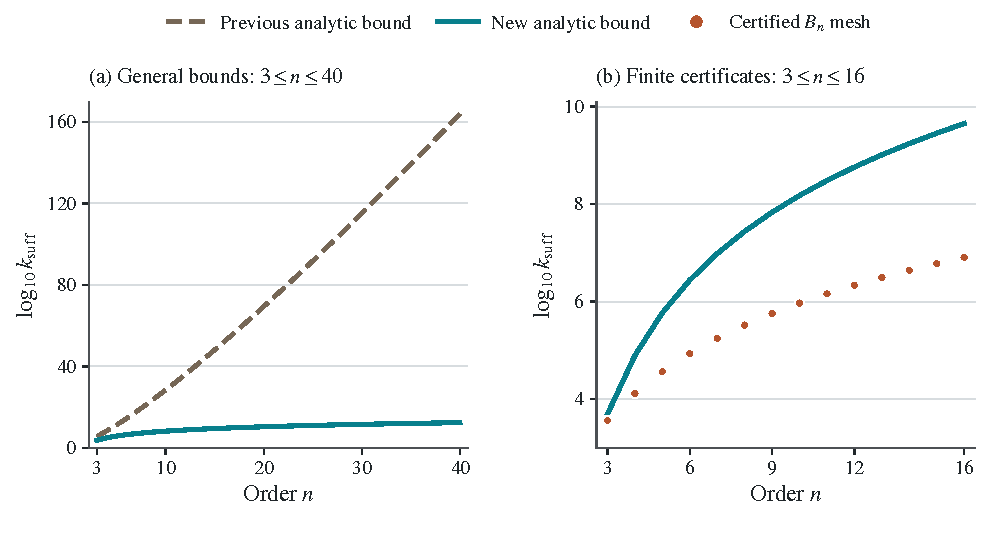
\includegraphics[width=\textwidth]{figures/lerch_thresholds.pdf}
\caption{Uniform sufficient bounds for Lerch zero saturation.
Panel (a) compares the earlier
$576n^2(3n)^{2n-4}$~\cite{incoming-uniform} with the new
$\mathcal K_n$ from \eqref{polylerch:eq:threshold}.
Panel (b) compares $\mathcal K_n$ with the smaller bounds obtained
from exact certified meshes of $B_n$. The vertical coordinates are
base-ten logarithms. Every displayed quantity is a sufficient bound;
no sharpness assertion is made.}
\label{audit:fig:thresholds}
\end{figure}

The Euler diagnostic program checks the derivative polynomials
symbolically and evaluates the positive integral remainder
$M_N(b)$ at high precision. Table~\ref{audit:tab:axis} illustrates
the axis optimization; its numbers are numerical approximations,
not interval-certified maximizers.

\begin{table}[tbp]
\centering\small
\begin{tabular}{@{}rrrr@{}}
\toprule
$N$ & Axis maximizer $b_N$ & $A_N-1$ & $N^p(A_N-1)$\\
\midrule
2 & $3.239719039892$ & $3.9230434864\,10^{-2}$ & $0.12830$\\
10 & $6.746559248034$ & $3.2851480198\,10^{-3}$ & $0.16829$\\
100 & $12.331892789531$ & $6.8858193177\,10^{-5}$ & $0.18071$\\
$10^4$ & $23.792066269001$ & $2.5107487089\,10^{-8}$ & $0.17292$\\
$10^{12}$ & $69.281926034579$ & $5.1420139643\,10^{-22}$ & $0.167984320879$\\
\bottomrule
\end{tabular}
\caption{Numerical axis optimization using the positive centered
integral. Full working values are supplied in
\src{data/late_euler_optimizers.csv}. Only the last row lies beyond
the explicit global axis-reduction threshold.}
\label{audit:tab:axis}
\end{table}

The second asymptotic scale converges much more slowly than the
leading normalized maximum. For example, at the leading maximizing
location $B\log N+d_0$, the diagnostic
$N^I\sqrt{\log N}\,M_N$ is still approximately $1.45355$ at
$N=10^{10000}$, whereas its proved limit is
$D=1.56777020071\ldots$. The small exponent
$4-(2B-1)=5-2B>0$ in the limiting positive tail explains why
the dominated-convergence proof can coexist with this slow approach.
The second term should therefore not be substituted into a rigorous
finite-$N$ error budget without an additional effective remainder
estimate.

\subsection{Further research questions and concrete conjectures}

\paragraph{1. A shorter tetralogarithm derivation.}
Can the forty-two-row tensor certificate be decomposed into a small
number of standard Kummer functional-equation substitutions?
This would make the proof easier to recognize in the classical
literature. The exact relation is established already; minimality
is a separate optimization problem. A systematic library of
real-branch descent certificates should record rational prime
contents, argument factorizations, endpoint values, and permitted
crossings.

\paragraph{2. Higher-weight golden and Gaussian identities.}
Apply the certificate method to the specific higher golden
reconstructions, with their endpoint logarithms and higher-weight
compatibility conditions made explicit. For the Gaussian problem,
seek an exact certificate for $S_6$ before enlarging the conjectural
$S_{2m}$ family. A useful success criterion is an explicit rational
relation in a stated functional-equation space whose analytic
evaluation can be proved. A smaller numerical residual or formal
rank calculation alone does not meet that criterion.

\paragraph{3. Is global axis reduction valid at every later index?}
The following strengthens the eventual theorem:
\begin{conjecture}[Axis reduction at every $N\ge2$]
\label{research:conj:allaxis}
For every integer $N\ge2$,
\[
 \sup_{a,b>0}R_N(a,b)=\max_{b>0}R_N(0,b).
\]
Every positive outer order gives a strict inequality.
\end{conjecture}
The axis maximum and its uniqueness are already proved for each such
$N$. What is missing is a global comparison over the positive
quadrant at the smaller indices. A proof need not show that
$R_N(a,b)$ decreases in $a$ for every $a,b$: that stronger
pointwise statement is not used by the present argument.
Validated compact optimization, joined to analytic estimates on all
noncompact parameter regions, could also reduce the explicit
threshold substantially.

\paragraph{4. Effective second-scale asymptotics and near maximizers.}
Obtain an explicit error estimate for
\eqref{lateaxis:eq:second}, and develop the inverse-$\log N$
corrections multiplying $N^{-I}/\sqrt{\log N}$. The centered
integral suggests coefficients involving derivatives of
$\Gamma(1/2-B)$. One must control the positive tail uniformly
before integrating an expanded density. Determine also the
sharp scale of the outer order among near maximizers; the proved
bound in Corollary~\ref{lateaxis:cor:concentration} is a necessary
concentration estimate, not an optimal local expansion in $a$.

\paragraph{5. The reversal order near outer order one.}
For each fixed $b>0$, the theorem implies
$\nu(a,b)\to\infty$ as $a\uparrow1$. Balancing the generic
$N^{-1/2}$ difference and the critical $N^{-1}$ difference leads
to the following precise candidate.
\begin{conjecture}[Near-critical reversal scale]
\label{research:conj:crossing}
For fixed $b>0$, with $\varepsilon=1-a\downarrow0$,
\[
 \nu(1-\varepsilon,b)\sim
 \frac{\bigl(\log(1/\varepsilon)\bigr)^{2b+2}}
 {\pi b^2\Gamma(b+1)^2\zeta(b+1)^2\,\varepsilon^2}.
\]
\end{conjecture}
The heuristic balance is
\[
 \varepsilon b\zeta(b+1)\sqrt\pi\,\Gamma(b+1)\sqrt N
 \asymp L^{b+1},\qquad L=\tfrac12\log N.
\]
It uses $1/\Gamma(-\varepsilon)\sim-\varepsilon$ and
$L\sim\log(1/\varepsilon)$ at the proposed crossing.
This is a newly proposed asymptotic, not a consequence of exchanging
limits in the fixed-parameter theorems. A proof needs a joint
expansion that retains both terms uniformly as $a\uparrow1$.
Quantitative asymptotics for the derivative zero sequence
$\nu_r$ from Corollary~\ref{phasefrac:cor:derivatives} form a
related problem.

\paragraph{6. Optimal truncation and exponentially small Euler terms.}
For integral $b=m$ and nonintegral $a$, the coefficient law
\eqref{frac:eq:largecoefficient} identifies the factorial growth
of the logarithmic series. Determine the optimal truncation index,
a rigorous remainder near that index, and its relation to the
exponentially small density terms discarded in the algebraic
large-$T$ expansion. Near integral $a$, the factor $\sin(\pi a)$
vanishes; any uniform result must resolve the transition from a
divergent expansion to an exactly terminating one.

\paragraph{7. Better Appell mesh and the least Lerch threshold.}
Can the explicit $n^{-3}$ gap be improved to $cn^{-2}$, or to
a different optimal scale? The auxiliary factor
$R_n(x)=\sum e_r x^r/(r+1)!$ provides a rational route to this
question. A stronger uniform mesh estimate immediately improves
the sufficient derivative order through
$\lceil(16+24H_{n-1}/\delta_n)^2\rceil$.
The elementary endpoint gives the necessary condition
$k\ge n-1$ for uniform simplicity; determine whether that condition
is also sufficient. It is important to separate saturation in
number from simplicity at the endpoint $\rho=0$.

\paragraph{8. Signed concentration and uniform higher zero offsets.}
The present proof controls an absolute logarithmic moment and gives
relative error $O(k^{-1/2})$. Cancellations in signed moments should
permit sharper location estimates. Develop them while $n$ grows
with $k$ and $\rho$ ranges over the full closed interval. Fixed-index
offset formulas in the manuscript are useful starting points, but
their constants must be controlled with respect to $n$ before a
growing-index conclusion is drawn.


\clearpage
\begin{thebibliography}{99}
\small
\raggedright
\addcontentsline{toc}{section}{References}

\bibitem{baseline}
ProveIt project, maintained by V.~Reshetnikov,
\emph{Polylogarithms manuscript and incoming research archives},
GitHub revision
\texttt{4c173c06cc32c9cea554b39be1837ad2ae897fc1},
10 October 2026.
Principal manuscript files used:
\src{03-algebraic.tex},
\src{05-real-euler.tex},
\src{05-subcritical-stieltjes.tex},
\src{05-signed-kernels.tex},
\src{05-universal-euler.tex}, and
\src{09-zero-geometry.tex}.
\url{https://github.com/VladimirReshetnikov/ProveIt/tree/4c173c06cc32c9cea554b39be1837ad2ae897fc1/Analysis/Polylogarithms/docs/manuscript}.
Archive inventory:
\url{https://github.com/VladimirReshetnikov/ProveIt/tree/4c173c06cc32c9cea554b39be1837ad2ae897fc1/docs/incoming}.

\bibitem{incoming-bounds}
ProveIt research continuation,
\emph{Polylogarithms: Uniform Bounds and Structural Transitions},
10 October 2026.
Source archive
\src{ProveIt_Polylogarithms_Research_2026-10-10.zip}
in \src{docs/incoming} at the revision in \cite{baseline}.
Relevant members:
\src{polylogarithms_uniform_bounds_20261010/sections/euler.tex}
and \src{sections/research.tex};
the latter contains \src{conj:euler-rate}.
The archive SHA256 and full member paths are in the source manifest.

\bibitem{incoming-uniform}
ProveIt research continuation,
\emph{Sharp Euler Bounds and Uniform Asymptotics in Polylogarithmic
Analysis: Reflected Moments, Lerch Zeros, and Integral Shuffle Lattices},
10 October 2026.
Source archive
\src{proveit_polylogarithms_research_2026-10-10 (1).zip}
in \src{docs/incoming} at the revision in \cite{baseline}.
Relevant members in \src{polylogarithms_uniform_continuation/sections}:
\src{04_lerch.tex}, \src{05_shuffle_and_identities.tex},
\src{06_review_and_corrections.tex}, and
\src{08_research_agenda.tex}.
The earlier explicit threshold is \src{efflerch:eq:Kn}.

\bibitem{incoming-sharp}
ProveIt research continuation,
\emph{The Sharp Universal Euler Constant for Harmonic Polylogarithms},
10 October 2026.
Source archive \src{ProveIt_Sharp_Universal_Euler_2026-10-10.zip}
in \src{docs/incoming} at the revision in \cite{baseline}.
Its positive divided-difference formula and certified universal constant
justify the common strict bound $R_N<57/50$ used by the finite
interval calculations. The corresponding integrated manuscript
section is \src{05-universal-euler.tex}.

\bibitem{Reshetnikov2015}
V.~Reshetnikov,
\emph{A conjectured identity for tetralogarithms $\operatorname{Li}_4$},
Mathematics Stack Exchange, question 1373123, 25 July 2015.
The original question states the six-argument formula; the 2017
answer by B.~W.~J.~Irwin proposes a Kummer-based route.
Accessed 10 October 2026.
\url{https://math.stackexchange.com/questions/1373123/}.

\bibitem{Reshetnikov2017}
V.~Reshetnikov,
\emph{Several conjectured identities for polylogarithms},
MathOverflow, question 261408, 5 February 2017.
The later answer by T.~Piezas III discusses the distinct golden
weight-five ladder formulas. Accessed 10 October 2026.
\url{https://mathoverflow.net/questions/261408/}.

\bibitem{polylerch:KSV}
O.~Katkova, B.~Shapiro, and A.~Vishnyakova,
\emph{Multiplier sequences and logarithmic mesh},
C.~R.~Math.~Acad.~Sci.~Paris \textbf{349} (2011), nos.~1--2, 35--38.
\url{https://doi.org/10.1016/j.crma.2010.11.031}.
Primary preprint: arXiv:1010.6052.
\url{https://arxiv.org/html/1010.6052v1}.
The paper states both the Riesz--Stoyanoff additive mesh result
and logarithmic mesh preservation for diagonal multipliers.

\bibitem{DLMFHurwitz}
F.~W.~J.~Olver et al., eds.,
\emph{NIST Digital Library of Mathematical Functions},
Chapter 25, \S25.11, Hurwitz zeta function.
Used for the continuation and recurrence conventions; the compensated
integral required here is derived in the text.
Accessed 10 October 2026.
\url{https://dlmf.nist.gov/25.11}.

\bibitem{DLMFGamma}
F.~W.~J.~Olver et al., eds.,
\emph{NIST Digital Library of Mathematical Functions},
Chapter 5, \S5.7, gamma-function series expansions.
Used for the logarithmic gamma coefficient conventions.
Accessed 10 October 2026.
\url{https://dlmf.nist.gov/5.7}.

\end{thebibliography}

\end{document}
